% Transcribed from blueprint/src/parts/03-pyramid.tex.
\section{A pyramid in $\RR^d$}
\label{ch:pyramid}

The introduction read a pyramid as a scale space sampled at the knots $q^n$. To use that reading
one must know which families a pyramid can sample, and how much of a family its ladder fixes. This
section settles both in $\RR^d$, $d \ge 1$, before any particular family is chosen.

The axiom is covariance under one dilation ratio $q > 1$. A pyramid here is a symmetric family of
kernels, continuous in scale, in which, after a relabelling of the scales, the kernel at scale
$q^nt$ is the kernel at $t$ dilated by $q^n$. Scale-space theory requires the same for every ratio
in place of $q$, and under that stronger axiom the families are classified, on the line and, with
rotation invariance, in $\RR^d$. One ratio is a weaker requirement, so it admits more families. The
first task is to see how many more, and how they are organized.

The families are organized by how much covariance they have. The ratios under which a family is covariant
always form a group, and only three kinds of group occur: the ratio $1$ alone, the powers of one
ratio, or all ratios. Fixing $q$, this sorts the families into three nested classes, the
\emph{strata}. Stratum~1 holds every symmetric family, covariant or not. Lindeberg's discrete scale space is
one of them. Stratum~2 holds the families covariant under $q$, the pyramids of this paper. Stratum~3
holds the families covariant under every ratio, those of classical scale-space theory. For
isotropic families each stratum has a plain description in \Levy{} coordinates, and an isotropic
example separates each stratum from the next.

The second task concerns what a pyramid computes. It applies the octave step from one knot to the
next and stores nothing in between. So the question is how much of the family the ladder of these
steps determines. It determines the kernels at the knots, but in general not the laws between
them. The same analysis says which laws can be steps at all, and it excludes the finite masks of
the classical pyramids.

The section runs as follows.
\begin{itemize}
\item Section~\ref{sec:pyramid-families} sets out the axioms, shows that the ratios of a family form
a closed group, and names the knots, the octave steps and the ladder.
\item Section~\ref{sec:pyramid-strata} defines the strata, describes them in \Levy{} coordinates
for isotropic families, and separates them by two examples. For a symmetric family that is not
isotropic, stratum~2 has the same description (Lemma~\ref{lem:discrete-covariance-levy}), and
stratum~3 is not described here.
\item Section~\ref{sec:pyramid-reduction} says what the reduction to the line keeps under one ratio,
and what it loses.
\item Section~\ref{sec:pyramid-ladder} shows that the ladder determines the knot kernels, and says
which laws are steps of a pyramid.
\item Section~\ref{sec:pyramid-bounded} excludes the steps of bounded support.
\end{itemize}
Section~\ref{sec:line-theory} reads the results at $d = 1$, and Section~\ref{supp:strata} of the
supplement restates them in the line's own terms.

Much of the machinery is probability theory. There a family continuous in scale is the system of
laws of the increments of an \emph{additive process in law}, a process with independent increments
that is continuous in probability [\sscite{sato1999levy}, \S 9]. Two-parameter families of laws
with the cascade are called convolution hemigroups, and Becker-Kern treats those covariant under a
linear map, at every ratio and at the powers of one ratio [\sscite{becker-kern2003stable}, p.~574].
This section proves what the pyramids need in the form they use it. Where a statement is a known
theorem for processes, the text before it names the theorem.

\subsection{Families and their dilations}
\label{sec:pyramid-families}

This subsection sets out the objects and proves the one structural fact that the rest of the section
builds on: the ratios under which a family is covariant form a closed group. Along the way it shows
that every step of a family is infinitely divisible, which is what brings \Levy{} data into the
theory.

The axioms are those of the isotropic paper, with two changes. Covariance is required at one
dilation only. Rotation invariance is kept apart from the other axioms, because pyramids computed
on a grid give it up. In $d \ge 2$, an exact pyramid computed on a lattice by one mask is never
isotropic (Proposition~\ref{prop:grid-pyramid-not-isotropic}, Section~\ref{ch:price}). What the
theory does need is symmetry. It makes every Fourier transform real. With the cascade it also makes
them positive, so each kernel has a real exponent $\Psi_t$ (Lemma~\ref{lem:family-structure}). The
transform $\widehat\mu$, the image $A_*\mu$ and the dilation $D_c$ are those of
Section~\ref{subsec:cited-notation}.

% shared with blueprint def:family-dimension-d
\begin{definition}[families in dimension $d$, and covariance under one dilation]
\label{def:family-dimension-d}

Let $d \ge 1$. A \emph{family in dimension $d$} is a family $(\mu_{s,t})_{0 \le s \le t}$ of
probability measures on $\RR^d$ with
\begin{itemize}
\item[(I1)] $\mu_{t,t} = \delta_0$, and $\mu_{r,t} = \mu_{s,t} * \mu_{r,s}$ for $r \le s \le t$
(cascade);
\item[(I2)] $(s,t) \mapsto \widehat\mu_{s,t}(\omega)$ continuous on $\{0 \le s \le t\}$ for each
$\omega \in \RR^d$ (continuity);
\item[(ND)] $\mu_{s,t} \ne \delta_0$ for $s < t$ (nondegeneracy).
\end{itemize}
The family is \emph{isotropic} if it also has
\begin{itemize}
\item[(I3)] $Q_*\mu_{s,t} = \mu_{s,t}$ for every $Q \in \Orth(d)$ and every pair,
\end{itemize}
and \emph{symmetric} if every $\mu_{s,t}$ is invariant under $x \mapsto -x$. For $\lambda > 0$ the
family is \emph{$\lambda$-covariant} if some increasing bijection $S_\lambda$ of $[0,\infty)$ has
$D_\lambda\mu_{s,t} = \mu_{S_\lambda s, S_\lambda t}$ for all $s \le t$. Write
$\mu_t := \mu_{0,t}$, the \emph{kernel} at scale $t$.
\end{definition}

In the labels of \prog{iso v0.1}{Def.~3.2, p.~11}, isotropy is (I3), and $\lambda$-covariance is
(I4) required at the one dilation $\lambda$. Isotropy implies symmetry, so every statement about
symmetric families applies to isotropic ones.

% shared with blueprint lem:isotropic-symmetric
\begin{lemma}[an isotropic family is symmetric]
\label{lem:isotropic-symmetric}

An isotropic family in dimension $d$ is symmetric.
\end{lemma}

\begin{proof}
The map $x \mapsto -x$ is $-I$, which lies in $\Orth(d)$. So (I3) at $Q = -I$ gives
$(-I)_*\mu_{s,t} = \mu_{s,t}$ for every pair, which is the symmetry of $\mu_{s,t}$.

Every step is machine-checked, with no cited fact.
\end{proof}

Before any covariance enters, the cascade and continuity already constrain each step. By the
cascade, a step is the convolution of arbitrarily many short steps. By continuity in scale, each
short step is close to $\delta_0$. A law that is such a limit is infinitely divisible. This needs
neither symmetry nor (ND). For the increments of an additive process in law it is Sato's theorem
[\sscite{sato1999levy}, Thm.~9.1, p.~47, and Thm.~9.7(i), p.~51].

% shared with blueprint lem:steps-infinitely-divisible
\begin{lemma}[the steps of a family are infinitely divisible]
\label{lem:steps-infinitely-divisible}

Let $d \ge 1$, and let $(\mu_{s,t})_{0 \le s \le t}$ be probability measures on $\RR^d$ with (I1)
and (I2). Then every $\mu_{s,t}$ is infinitely divisible.
\end{lemma}

\begin{proof}
By (I2) and \Levy's continuity theorem, $(s,t) \mapsto \mu_{s,t}$ is weakly continuous on
$\{0 \le s \le t\}$. Short steps are therefore uniformly close to $\delta_0$ on bounded sets of
scales: for $T > 0$ and $\varepsilon, \eta > 0$ there is $\delta > 0$ with
$\mu_{u,v}(\{|x| \ge \varepsilon\}) < \eta$ whenever $u \le v \le T$ and $v - u < \delta$. Otherwise
there is a sequence $(u_k, v_k)$ with $v_k \le T$, $v_k - u_k \to 0$ and
$\mu_{u_k,v_k}(\{|x| \ge \varepsilon\}) \ge \eta$. A subsequence converges to some $(u_0, u_0)$, and
the portmanteau theorem for the closed set $\{|x| \ge \varepsilon\}$ gives
$\eta \le \mu_{u_0,u_0}(\{|x| \ge \varepsilon\}) = 0$, since $\mu_{u_0,u_0} = \delta_0$ by (I1).

Fix $s < t$, and let $s = t_0 < t_1 < \dots < t_n = t$ be the partition into $n$ equal parts. By
(I1), $\mu_{s,t} = \mu_{t_{n-1},t} * \dots * \mu_{t_0,t_1}$. Take independent random vectors
$X_{n,1}, \dots, X_{n,n}$ with the laws $\mu_{t_{j-1},t_j}$. By the previous paragraph
$\max_jP(|X_{n,j}| \ge \varepsilon) \to 0$ as $n \to \infty$ for every $\varepsilon > 0$, so the
$X_{n,j}$ form a null array. Each row sum has the law $\mu_{s,t}$. So the row sums converge in law to
$\mu_{s,t}$, which is infinitely divisible by Khintchine's theorem
(Theorem~\ref{thm:cited-A41}). For $s = t$ the law $\delta_0$ is infinitely divisible.

Every step is machine-checked, and the cited fact is \ledger{A41}.
\end{proof}

A symmetric infinitely divisible law has a real exponent, given by a Gaussian part and a
symmetric \Levy{} measure. This is the symmetric form of the \Levy--Khintchine theorem, and it has
a converse. The paper uses it for the kernels of a family, for the masks of a pyramid and for their
knot kernels.

% shared with blueprint lem:symmetric-levy-khintchine
\begin{lemma}[the symmetric \Levy--Khintchine form]
\label{lem:symmetric-levy-khintchine}

A probability measure $\mu$ on $\RR^d$ is symmetric and infinitely divisible if and only if
\[
  \widehat\mu(\omega) = \exp\Bigl(-\langle\omega, A\omega\rangle
  - \int\bigl(1 - \cos\langle\omega, x\rangle\bigr)\,\nu(dx)\Bigr), \qquad \omega \in \RR^d,
\]
for a positive semidefinite $d \times d$ matrix $A$ and a symmetric measure $\nu$ on $\RR^d$ with
$\nu(\{0\}) = 0$ and $\int\min(|x|^2, 1)\,\nu(dx) < \infty$. The pair $(A, \nu)$ is then unique. It
is the \emph{\Levy{} data} of $\mu$, with \emph{Gaussian part} $A$ and \emph{\Levy{} measure} $\nu$,
and $\mu$ has the generating triplet $(2A, \nu, 0)$.
\end{lemma}

\begin{proof}
\emph{Only if.} Let $\mu$ be symmetric and infinitely divisible. By the \Levy--Khintchine theorem
(Theorem~\ref{thm:cited-A39}(i)) it has a generating triplet $(A^{\mathrm S}, \nu, \gamma)$, with
\[
  \widehat\mu(\omega) = \exp\Bigl[-\tfrac12\langle\omega, A^{\mathrm S}\omega\rangle + i\langle\gamma, \omega\rangle
  + \int\bigl(e^{i\langle\omega, x\rangle} - 1 - i\langle\omega, x\rangle\mathbf 1_{\{|x| \le 1\}}\bigr)\,\nu(dx)\Bigr],
\]
and the triplet is unique (Theorem~\ref{thm:cited-A39}(ii)). The change of variables
$x \mapsto -x$ in this formula shows that the reflected law has the triplet
$(A^{\mathrm S}, \nu(-\,\cdot), -\gamma)$, the unit ball being symmetric. A symmetric law equals its
reflection, so uniqueness gives $\gamma = 0$ and $\nu$ symmetric. The odd part
$i\sin\langle\omega, x\rangle - i\langle\omega, x\rangle\mathbf 1_{\{|x| \le 1\}}$ of the integrand
is absolutely integrable against $\nu$, as $|\sin y - y| \le |y|^3/6$ and $\nu$ is finite off the
unit ball. So it integrates to $0$ against the symmetric $\nu$. What is left is the displayed form,
with $A := \tfrac12A^{\mathrm S}$, the Gaussian part in the normalization of
Section~\ref{subsec:cited-notation}.

\emph{If.} Let $\widehat\mu$ have the displayed form. The computation above, read backwards with
$\gamma = 0$ and $\nu$ symmetric, shows that $\widehat\mu$ is given by the formula of
Theorem~\ref{thm:cited-A39}(i) with the triplet $(2A, \nu, 0)$. By Theorem~\ref{thm:cited-A39}(iii)
some infinitely divisible law has that transform. A law is determined by its transform, so $\mu$ is
that law, and it is infinitely divisible. Its transform is real. The reflection of $\mu$ has the
conjugate transform, which is the same, so $\mu$ is symmetric.

\emph{Uniqueness.} If $(A, \nu)$ and $(A', \nu')$ are both data of $\mu$, then $(2A, \nu, 0)$ and
$(2A', \nu', 0)$ are both generating triplets of $\mu$, as in the previous paragraph. So
Theorem~\ref{thm:cited-A39}(ii) gives $A = A'$ and $\nu = \nu'$.

Every step is machine-checked, and the cited fact is \ledger{A39}.
\end{proof}

With symmetry more follows. Every transform is real and positive, so each kernel has a real
exponent. Its \Levy{} data, a Gaussian part and a \Levy{} measure, grow with scale, and the data of
a step are the difference of the data at its two ends. The next lemma is used throughout the paper.
For an additive process in law, Sato describes the laws by such a system of data, which vanish at
$0$, grow and are continuous, and he proves the converse [\sscite{sato1999levy}, Thm.~9.8, p.~52].
The lemma is the symmetric case of that description, read on a family, and
Theorem~\ref{thm:lattice-strata}(1) is the converse in the isotropic case.

% shared with blueprint lem:family-structure
\begin{lemma}[structure]
\label{lem:family-structure}

Let $(\mu_{s,t})$ be a symmetric family in dimension $d$. Each $\mu_{s,t}$ is infinitely divisible
with $\widehat\mu_{s,t} > 0$. With $\Psi_t := -\log\widehat\mu_t$ one has
$\widehat\mu_{s,t} = e^{-(\Psi_t - \Psi_s)}$ and
\[
  \Psi_t(\omega) = \langle\omega, A_t\omega\rangle + \int\bigl(1 - \cos\langle\omega, x\rangle\bigr)\,\nu_t(dx),
\]
with $A_t$ and $\nu_t$ nondecreasing in $t$, $A_t$ in the order of positive semidefinite matrices
and $\nu_t$ setwise, and $\mu_{s,t}$ has the data $(A_t - A_s, \nu_t - \nu_s)$.
The map $t \mapsto \mu_t$ is injective, and $t \mapsto \widehat\mu_t(\omega)$ is nonincreasing. If
the family is isotropic, $A_t = a(t)I$ and $\nu_t$ is rotation invariant.
\end{lemma}

\begin{proof}
Each $\mu_{s,t}$ is infinitely divisible by Lemma~\ref{lem:steps-infinitely-divisible}.
The transform of an infinitely divisible law has no zero (Theorem~\ref{thm:cited-A40}).
The transform of a symmetric law is real. So $\widehat\mu_{s,t}$ is real, continuous and without
zeros on the connected set $\RR^d$, with $\widehat\mu_{s,t}(0) = 1$, hence positive. By (I1) with
$r = 0$, $\widehat\mu_t = \widehat\mu_{s,t}\widehat\mu_s$, so
$\widehat\mu_{s,t} = e^{-(\Psi_t - \Psi_s)}$.

Each $\mu_t$ and each $\mu_{s,t}$ is symmetric and infinitely divisible, so it has unique
\Levy{} data by Lemma~\ref{lem:symmetric-levy-khintchine}: $(A_t, \nu_t)$ for $\mu_t$, which gives
$\Psi_t$ the displayed form, and $(A_{s,t}, \nu_{s,t})$ for $\mu_{s,t}$. The exponent
$\Psi_t = \Psi_s + (\Psi_t - \Psi_s)$ is the sum of the exponents of $\mu_s$ and $\mu_{s,t}$, so it
is of the same form with the data $(A_s + A_{s,t}, \nu_s + \nu_{s,t})$. Uniqueness gives
$A_t = A_s + A_{s,t}$ and $\nu_t = \nu_s + \nu_{s,t}$. So $A_t - A_s = A_{s,t}$ is positive semidefinite,
$\nu_t - \nu_s = \nu_{s,t}$ is a positive measure, and $\mu_{s,t}$ has the data
$(A_t - A_s, \nu_t - \nu_s)$. Since $\Psi_t - \Psi_s$ is the exponent of $\mu_{s,t}$, it is
nonnegative, and $\widehat\mu_t(\omega)$ is nonincreasing in $t$.

If $\mu_t = \mu_{t'}$ with $t < t'$, then $\widehat\mu_{t,t'} = \widehat\mu_{t'}/\widehat\mu_t = 1$,
so $\mu_{t,t'} = \delta_0$, against (ND).

Let the family be isotropic and $Q \in \Orth(d)$. The image $Q_*\mu_t$ of the infinitely divisible
law $\mu_t$ has the Gaussian datum $QA_tQ^{\tp}$ and the \Levy{} measure $Q_*\nu_t$
(Theorem~\ref{thm:cited-A42}). That theorem restricts the image of $\nu_t$ to
$\RR^d \setminus \{0\}$, which changes nothing here, since $Q$ is injective and $\nu_t\{0\} = 0$.
Since $Q_*\mu_t = \mu_t$, uniqueness gives $QA_tQ^{\tp} = A_t$ and $Q_*\nu_t = \nu_t$. Take for $Q$
the diagonal matrix that changes the sign of the $j$-th coordinate. Then
$(QA_tQ^{\tp})_{jk} = -(A_t)_{jk}$ for $k \ne j$, so the entries of $A_t$ off the diagonal vanish.
Take for $Q$ the permutation matrix that exchanges the first and the $k$-th coordinate. Then
$(A_t)_{kk} = (A_t)_{11}$. So $A_t = a(t)I$ with $a(t) := (A_t)_{11}$.

Every step is machine-checked, and the cited facts are \ledger{A40}, \ledger{A39} and
\ledger{A42}, with \ledger{A41} through Lemma~\ref{lem:steps-infinitely-divisible}.
\end{proof}

The pair $(A_t, \nu_t)$ is the \Levy{} data of $\mu_t$ in the sense of
Lemma~\ref{lem:symmetric-levy-khintchine}. The \Levy{} measure is the rate of the jumps of each size and
direction [\sscite{sato1999levy}, Thm.~19.2(i), p.~120].

Covariance enters now. Under which ratios $\lambda$ is a given family covariant? The next lemma
shows that the answer is always a closed group, so that only three kinds of answer occur. It also
shows that a family covariant under $q$ can be relabelled in scale so that its bijection is
$t \mapsto qt$. Most later statements are made in this canonical gauge. For a semi-selfsimilar
process, Maejima and Sato prove a dichotomy of the same kind for its \emph{epochs}, the time
factors $a > 1$ under which it rescales to itself in law: they are the powers of one number, or
all of $(1,\infty)$ [\sscite{maejima1999semi}, Thm.~1(ii), p.~349]. Here the group consists of
ratios in space and the change of scale is arbitrary, so the lemma is proved in full.

% shared with blueprint lem:family-dilations
\begin{lemma}[the dilations of a family]
\label{lem:family-dilations}

Let $(\mu_{s,t})$ be a symmetric family in dimension $d$, and let $G$ be the set of $\lambda > 0$ for
which it is $\lambda$-covariant.
\begin{enumerate}
\item For $\lambda \in G$ the bijection $S_\lambda$ is unique, and $S_\lambda t > t$ for all $t > 0$
when $\lambda > 1$.
\item $G$ is a closed subgroup of $(0,\infty)$. So $G$ is $\{1\}$, some $q^{\ZZ}$ with $q > 1$, or
$(0,\infty)$.
\item If $q \in G$ with $q > 1$, there is an increasing homeomorphism $\chi$ of $[0,\infty)$ with
$\chi S_q = q\chi$. The relabelled family $(\mu_{\chi^{-1}s,\chi^{-1}t})$ then has $S_qt = qt$, the
\emph{canonical discrete gauge}. Two choices of $\chi$ differ by an element of the group
$\mathcal{G}_q$ of increasing homeomorphisms $g$ of $(0,\infty)$ with $g(qt) = q\,g(t)$, each
extended to $[0,\infty)$ by $g(0) := 0$.
\item (The line.) In particular, a symmetric family in dimension $1$ that is $q$-covariant for some
$q > 1$ has a bijection $S_q$ with no fixed point in $(0,\infty)$, and after the relabelling of (3)
it has the canonical discrete gauge $S_qt = qt$, unique up to $\mathcal{G}_q$.
\end{enumerate}
\end{lemma}

\begin{proof}
(1) Since $S_\lambda$ is an increasing bijection of $[0,\infty)$, $S_\lambda0 = 0$, so
$D_\lambda\mu_t = \mu_{S_\lambda t}$. If $S$ and $S'$ both serve, then $\mu_{St} = \mu_{S't}$, and
$St = S't$ by the injectivity of Lemma~\ref{lem:family-structure}. Put
$\phi_t := \widehat\mu_t > 0$, so that $\phi_{S_\lambda t}(\omega) = \phi_t(\lambda\omega)$. Let
$\lambda > 1$ and $t > 0$, and suppose that $S_\lambda t \le t$. Since $\phi_t$ is nonincreasing in
$t$ (Lemma~\ref{lem:family-structure}), $\phi_t(\lambda\omega) = \phi_{S_\lambda t}(\omega) \ge
\phi_t(\omega)$ for all $\omega$. Applied at $\lambda^{-1}\omega, \lambda^{-2}\omega, \dots$ this
gives $\phi_t(\omega) \ge \phi_t(\lambda^{-n}\omega)$ for $n \ge 0$, and $n \to \infty$ gives
$\phi_t(\omega) \ge \phi_t(0) = 1$, by the continuity of $\phi_t$. Since $\phi_t \le 1$, $\phi_t \equiv 1$,
so $\mu_t = \delta_0$, against (ND). Hence $S_\lambda t > t$.

(2) $G$ contains $1$. If $\lambda, \lambda' \in G$, then
$D_{\lambda\lambda'}\mu_{s,t} = D_\lambda\mu_{S_{\lambda'}s, S_{\lambda'}t} =
\mu_{S_\lambda S_{\lambda'}s, S_\lambda S_{\lambda'}t}$, and applying $D_{\lambda^{-1}}$ to
$D_\lambda\mu_{s,t} = \mu_{S_\lambda s, S_\lambda t}$ gives
$D_{\lambda^{-1}}\mu_{s',t'} = \mu_{S_\lambda^{-1}s', S_\lambda^{-1}t'}$. So $G$ is a group, with
$S_{\lambda\lambda'} = S_\lambda S_{\lambda'}$ and $S_{\lambda^{-1}} = S_\lambda^{-1}$.

The bijections increase with the ratio: if $a < b$ lie in $G$, then $S_at \le S_bt$ for $t \ge 0$.
Indeed $S_{a^{-1}}S_b$ serves $a^{-1}b > 1$, so by (1) $S_{a^{-1}}S_bt > t$ for $t > 0$, and
applying $S_a$ gives $S_bt > S_at$.

For closedness let $\lambda_n \in G$ with $\lambda_n \to \lambda > 0$. If $G$ has no element
above $1$, then, being closed under inverses, $G = \{1\}$, so every $\lambda_n$ is $1$ and
$\lambda = 1 \in G$. Otherwise $G$ contains some $g_0 > 1$ and its powers, so there is $g \in G$ with
$g > \lambda_n$ for all large $n$. Fix $t \ge 0$. Then $0 \le S_{\lambda_n}t \le S_gt$ for all
large $n$, and along a subsequence $S_{\lambda_n}t \to \tau \ge 0$. By (I2) and the continuity of
$\phi_t$,
\[
  \phi_\tau(\omega) = \lim_n\phi_{S_{\lambda_n}t}(\omega) = \lim_n\phi_t(\lambda_n\omega) = \phi_t(\lambda\omega).
\]
So $D_\lambda\mu_t = \mu_\tau$, and by injectivity $\tau$ is determined by $t$. Put
$S_\lambda t := \tau$. The same argument for $\lambda_n^{-1} \to \lambda^{-1}$, with
$\lambda_n^{-1} \in G$, gives $S'$ with $D_{\lambda^{-1}}\mu_t = \mu_{S't}$ for $t \ge 0$. Then
$\mu_{S_\lambda S't} = D_\lambda\mu_{S't} = \mu_t$ forces $S_\lambda S't = t$, so $S_\lambda$ maps
$[0,\infty)$ onto itself. It is strictly increasing: if $t < t'$ and $S_\lambda t' \le S_\lambda t$,
then
$\phi_t(\lambda\omega) = \phi_{S_\lambda t}(\omega) \le \phi_{S_\lambda t'}(\omega) = \phi_{t'}(\lambda\omega)
\le \phi_t(\lambda\omega)$ for all $\omega$, so $\phi_t = \phi_{t'}$ and $\mu_t = \mu_{t'}$, against
injectivity. So $S_\lambda$ is an increasing bijection of $[0,\infty)$. By
Lemma~\ref{lem:family-structure},
$\widehat\mu_{s,t} = \phi_t/\phi_s$, so
$\widehat\mu_{s,t}(\lambda\omega) = \phi_{S_\lambda t}(\omega)/\phi_{S_\lambda s}(\omega) =
\widehat\mu_{S_\lambda s, S_\lambda t}(\omega)$, and $\lambda \in G$.

The logarithm maps $G$ onto a closed subgroup $H$ of $(\RR, +)$. If $H \ne \{0\}$, let
$\ell := \inf(H \cap (0,\infty))$. If $\ell > 0$, then $\ell \in H$ since $H$ is closed, and every
$h \in H$ is an integer multiple of $\ell$, since $h - \lfloor h/\ell\rfloor\ell \in H \cap [0,\ell)$
is $0$. So $H = \ell\ZZ$ and $G = q^{\ZZ}$ with $q = e^\ell$. If $\ell = 0$, $H$ contains arbitrarily
small positive elements, so it is dense, and $H = \RR$ since it is closed.

(3) $S_q$ is continuous, being an increasing bijection of $[0,\infty)$, and $S_qt > t$ for $t > 0$
by (1). The increasing sequence $S_q^n1$ has no
finite limit, since a finite limit would be a fixed point of $S_q$, so $S_q^n1 \to \infty$. In the
same way the decreasing sequence $S_q^{-n}1$ tends to $0$. So every $t > 0$ lies in exactly one
interval $[S_q^n1, S_q^{n+1}1)$, $n \in \ZZ$. Let $\chi_0$ be any increasing bijection of
$[1, S_q1)$ onto $[1, q)$, for instance the affine one, and put $\chi(t) := q^n\chi_0(S_q^{-n}t)$ for
$t \in [S_q^n1, S_q^{n+1}1)$ and $\chi(0) := 0$. Then $\chi S_q = q\chi$, since $S_q$ maps
$[S_q^n1, S_q^{n+1}1)$ onto $[S_q^{n+1}1, S_q^{n+2}1)$. The map $\chi$ takes each interval
$[S_q^n1, S_q^{n+1}1)$ increasingly onto $[q^n, q^{n+1})$, so it is strictly increasing and maps
$[0,\infty)$ onto itself. An increasing map of $[0,\infty)$ onto itself has no jump, so $\chi$ is
continuous, and it is an increasing homeomorphism of $[0,\infty)$. For the relabelled family, $\chi^{-1}(qs) = S_q\chi^{-1}(s)$ gives
\[
  D_q\mu_{\chi^{-1}s, \chi^{-1}t} = \mu_{S_q\chi^{-1}s, S_q\chi^{-1}t} = \mu_{\chi^{-1}(qs), \chi^{-1}(qt)},
\]
and (I1), (I2) and (ND) pass to it because $\chi$ is an increasing homeomorphism. If $\chi'$ also has
$\chi'S_q = q\chi'$, then $g := \chi'\chi^{-1}$ is an increasing homeomorphism of $[0,\infty)$
with $g(0) = 0$, and $g(qt) = \chi'(S_q\chi^{-1}t) = q\chi'(\chi^{-1}t) = q\,g(t)$. So its
restriction to $(0,\infty)$ lies in $\mathcal{G}_q$, and $\chi' = g\chi$.

(4) is (1) and (3) at $d = 1$. A family on $\RR$ is read as one on $\RR^1$ through $x \mapsto xe_1$,
which keeps (I1), (I2), (ND), symmetry and the transforms, so the facts of
Lemma~\ref{lem:family-structure} used above hold on $\RR$.

Every step is machine-checked, and the cited facts enter only through
Lemma~\ref{lem:family-structure}.
\end{proof}

In the canonical gauge the scales $q^n$ play a special part. A pyramid stores its levels there,
and what it computes are the steps from one of these scales to the next. The next definition names
them, and Figure~\ref{fig:pyramid-schematic} shows them on the scale axis.

% shared with blueprint def:knots-and-ladder
\begin{definition}[knots, knot kernels and the ladder]
\label{def:knots-and-ladder}

Let $(\mu_{s,t})$ be a symmetric family in dimension $d$ that is $q$-covariant, $q > 1$, in the
canonical discrete gauge $S_qt = qt$ of Lemma~\ref{lem:family-dilations}(3). The scales $q^n$,
$n \in \ZZ$, are its \emph{knots}, the scales at which a pyramid stores a level. The kernels
$\mu_{q^n}$ are its \emph{knot kernels}. An \emph{octave} is a factor $q$ in scale, an interval
$[t, qt]$ with $t > 0$, and $\mu_{t,qt}$ is the \emph{octave step} across it. The sequence
$(\mu_{q^n,q^{n+1}})_{n \in \ZZ}$ of the octave steps between consecutive knots is its \emph{ladder}.
\end{definition}

The word octave is used for every ratio $q > 1$, not only for $q = 2$. One step
$\mu_{q^n,q^{n+1}}$ of the ladder is also called a \emph{rung}. By covariance
$\mu_{q^n,q^{n+1}} = D_{q^n}\mu_{1,q}$, so the whole ladder is one step $\mu_{1,q}$, dilated to
each level. The same words are used on a grid (Definition~\ref{def:exact-grid-pyramid}).

Which scale is called $1$ is a choice in $\mathcal{G}_q$, so the knots are fixed only up to a
relabelling. The ladder of a family fixes its knot kernels. It does not fix the laws between them.
It fixes them up to a relabelling exactly when the data of the step span an extreme ray of the cone
of data, the pairs $(A, \nu)$ with $A$ positive semidefinite and $\nu$ a symmetric \Levy{} measure.
A Gaussian step of rank one does, and so does a step whose jumps are $\pm x$ along one vector
(Proposition~\ref{prop:ladder-knot-kernel}(2)).

One more tool is needed before the strata. A pyramid on a grid applies a law carried by a lattice
at each step. The next lemma says that if such a law is infinitely divisible, it has no Gaussian
part and all its jumps land on the lattice. Sections~\ref{sec:pyramid-ladder} and~\ref{ch:price}
use it.

% shared with blueprint lem:lattice-infinitely-divisible
\begin{lemma}[lattice-carried infinitely divisible laws in $\RR^d$]
\label{lem:lattice-infinitely-divisible}

Let $\eta$ be an infinitely divisible law on $\RR^d$ with generating triplet $(A^{\mathrm S}, \nu, \beta)$,
carried by a full-rank lattice $\Gamma$. Then $A^{\mathrm S} = 0$, and $\nu$ is a finite measure carried by
$\Gamma \setminus \{0\}$.
\end{lemma}

\begin{proof}
Let $b_1, \dots, b_d$ be a basis of $\Gamma$ over $\ZZ$. It is a basis of $\RR^d$, and $\Gamma$ is the
set of points whose coordinates $c_1(x), \dots, c_d(x)$ in this basis are integers. Write
$c_i(x) = \langle v_i, x\rangle$.

Fix $i$. The image $\eta_i$ of $\eta$ under $c_i$ is an infinitely divisible law on $\RR$, with
Gaussian coefficient $\langle v_i, A^{\mathrm S}v_i\rangle$ and \Levy{} measure $\nu_i$, the image of $\nu$
under $c_i$ restricted to $\RR \setminus \{0\}$ (Theorem~\ref{thm:cited-A42}). Since $\eta$ is
carried by $\Gamma$, $\eta_i$ is carried by $\ZZ$, so its support lies in the closed set $\ZZ$. By
Theorem~\ref{thm:cited-A48}, $\langle v_i, A^{\mathrm S}v_i\rangle = 0$, and $\nu_i$ is finite and carried
by $\ZZ$.

Since $A^{\mathrm S}$ is positive semidefinite, $\langle v_i, A^{\mathrm S}v_i\rangle = 0$ gives $A^{\mathrm S}v_i = 0$. The vectors
$v_i$ span $\RR^d$: expanding $e_m$ in the basis gives $\sum_i(b_i)_k\,c_i(e_m) = (e_m)_k$, so
$e_k = \sum_i(b_i)_kv_i$. So $A^{\mathrm S} = 0$.

The set $\{x : c_i(x) \notin \ZZ\}$ does not contain $0$, so
$\nu(\{x : c_i(x) \notin \ZZ\}) = \nu_i(\RR \setminus \ZZ) = 0$ for every $i$. A point outside
$\Gamma$ has a coordinate outside $\ZZ$, so $\nu$ is carried by $\Gamma$, and by
$\Gamma \setminus \{0\}$, since a \Levy{} measure puts no mass at $0$. Finally, every $x \ne 0$ has
a nonzero coordinate, so
$\nu(\RR^d \setminus \{0\}) \le \sum_i\nu(\{x : c_i(x) \ne 0\}) = \sum_i\nu_i(\RR \setminus \{0\}) < \infty$.

Every step is machine-checked, and the cited facts are \ledger{A42} and \ledger{A48}.
\end{proof}

\subsection{Three nested strata}
\label{sec:pyramid-strata}

This subsection defines the strata and describes each of them by the \Levy{} data of its
families. The description turns covariance, a statement about kernels at different scales, into
scaling laws for the data. It also places the kernels of a pyramid among the laws of probability
theory. They are semi-selfdecomposable laws, which stand to one ratio as the self-decomposable laws
stand to every ratio.

A law is \emph{self-decomposable} if, for every $0 < c < 1$, it is the law of $cX + Y$ with $X$ of that
law and $Y$ independent of $X$ [\sscite{sato1999levy}, Def.~15.1, p.~90]
(Definition~\ref{def:self-decomposable}). Shrinking the law by any factor and adding independent
noise gives it back. These laws are the kernels of scale-space theory. On the line the kernels of the
fully covariant families at positive scales are exactly the symmetric self-decomposable laws other
than $\delta_0$ \prog{V-line v0.1}{Thm.~7.3, p.~37, with Prop.~2.13, p.~13}. In $\RR^d$, with
rotation invariance, they are exactly the rotation-invariant self-decomposable laws other than
$\delta_0$ \prog{iso v0.1}{Cor.~3.9(1), p.~14}, whose exponents are the $F(|\cdot|)$ with
$F \in \mathcal{A}_d$ (Theorem~\ref{thm:cited-A35}(2)).

Under one dilation the decomposition is required at the one factor $c = 1/q$ only, and Sato calls
the ratio $q$ a \emph{span}. Maejima and Naito require the remainder, the \emph{residual}, to be
infinitely divisible [\sscite{maejima1998semi}, Def.~3.1, p.~19, and Thm.~3.1(i), p.~20]. Theirs is the
semi-selfdecomposable class of Definition~\ref{def:self-decomposable}:
$\widehat\mu = \widehat\mu(q^{-1}\,\cdot)\,\widehat\varrho_q$ for some infinitely divisible law
$\varrho_q$. In a pyramid the residual is a dilate of an octave step, and every step is infinitely
divisible, so the requirement costs nothing there. Read upward, the decomposition is the knot
relation $D_q\mu = \mu * D_q\varrho_q$. So a law is semi-selfdecomposable with span $q$ exactly when
it is refinable at the ratio $q$, in the sense of Section~\ref{sec:pyramid-bounded}, with an
infinitely divisible mask. Without the requirement the class is wider, and
Section~\ref{sec:pyramid-bounded} shows a law of the wider class, the cubic B-spline, that is the
kernel of no family.

A semi-selfdecomposable law $\mu$ with span $q$ is infinitely divisible, and its residual
$\varrho_q$ is unique [\sscite{sato1999levy}, Prop.~15.5, p.~93] (Theorem~\ref{thm:cited-A43}).
The sentence after its proof makes a self-decomposable law semi-selfdecomposable for every span. Whether a
law is in the class can be read off its \Levy{} measure. An
infinitely divisible law with \Levy{} measure $\nu$ is semi-selfdecomposable with span $q$ iff
$D_q\nu \ge \nu$, with no condition on its Gaussian part [\sscite{sato1999levy}, Thm.~15.8,
p.~94] (Theorem~\ref{thm:cited-A44}). In words, dilating the jumps by $q$ must not lose any of
them.

The first lemma writes covariance under $q$ in \Levy{} coordinates. Covariance becomes two scaling
laws for the data, one for the Gaussian part and one for the \Levy{} measure.

% shared with blueprint lem:discrete-covariance-levy
\begin{lemma}[discrete covariance in \Levy{} coordinates]
\label{lem:discrete-covariance-levy}

Let $(\mu_{s,t})$ be a symmetric family in dimension $d$, with the data $(A_t, \nu_t)$ of
Lemma~\ref{lem:family-structure}, and let $q > 1$. The family is $q$-covariant with $S_qt = qt$ iff
$\Psi_{qt}(\omega) = \Psi_t(q\omega)$ for all $t \ge 0$ and $\omega \in \RR^d$, iff
\begin{equation}
\label{eq:discrete-covariance-levy}
  A_{qt} = q^2A_t, \qquad \nu_{qt} = D_q\nu_t \qquad \text{for all } t > 0.
\end{equation}
Every $\mu_t$ is then semi-selfdecomposable with span $q$, and the family is determined by its
kernels $\mu_t$, $t \in [1, q)$.
\end{lemma}

\begin{proof}
The transform of $D_q\mu$ is $\widehat\mu(q\,\cdot)$. If the family is $q$-covariant with
$S_qt = qt$, then at the pairs $(0, t)$ it gives $D_q\mu_t = \mu_{qt}$, which is
$\Psi_{qt}(\omega) = \Psi_t(q\omega)$. Conversely, if this holds, Lemma~\ref{lem:family-structure}
gives, for every pair,
$\widehat\mu_{s,t}(q\omega) = e^{-(\Psi_t(q\omega) - \Psi_s(q\omega))} =
e^{-(\Psi_{qt}(\omega) - \Psi_{qs}(\omega))} = \widehat\mu_{qs,qt}(\omega)$.

The change of variables $y = qx$ gives
\[
  \Psi_t(q\omega) = \langle\omega, q^2A_t\omega\rangle + \int\bigl(1 - \cos\langle\omega, y\rangle\bigr)\,D_q\nu_t(dy).
\]
Here $D_q\nu_t$ is a symmetric \Levy{} measure, since it puts no mass at $0$ and
$\int(1 \wedge |y|^2)\,D_q\nu_t(dy) = \int(1 \wedge q^2|x|^2)\,\nu_t(dx) \le q^2\int(1 \wedge |x|^2)\,\nu_t(dx)$.
So $\Psi_t(q\,\cdot)$ is the exponent with the data $(q^2A_t, D_q\nu_t)$, and by the uniqueness of the
generating triplet (Theorem~\ref{thm:cited-A39}(ii)) it equals $\Psi_{qt}$ iff
(\ref{eq:discrete-covariance-levy}) holds at $t$. At $t = 0$ both sides vanish.

Under covariance, $D_q\mu_t = \mu_{qt} = \mu_{t,qt} * \mu_t$, so
$\widehat\mu_t(q\omega) = \widehat\mu_t(\omega)\widehat\mu_{t,qt}(\omega)$. Replacing $\omega$ by
$q^{-1}\omega$ gives $\widehat\mu_t = \widehat\mu_t(q^{-1}\,\cdot)\,\widehat\varrho_q$ with the residual
$\varrho_q := D_{q^{-1}}\mu_{t,qt}$. It is infinitely divisible because $\mu_{t,qt}$ is, by
Lemma~\ref{lem:family-structure}, and the dilate of an $n$-th convolution root is an $n$-th
convolution root of the dilate. This is what Definition~\ref{def:self-decomposable} requires.
Finally, every $t > 0$ is $q^nt'$ with $n \in \ZZ$ and $t' \in [1, q)$, and covariance gives
$\mu_t = D_{q^n}\mu_{t'}$. Also $\mu_0 = \delta_0$, and every step is determined by
$\widehat\mu_{s,t} = \widehat\mu_t/\widehat\mu_s$.

Every step is machine-checked, and the cited facts are \ledger{A39}(ii)--(iii) and those of
Lemma~\ref{lem:family-structure}.
\end{proof}

So a $q$-covariant family is fixed by its data on one octave $[1, q)$. The converse builds a
family from such data. Any data on $[1, q]$ that grow strictly and continuously, and whose two ends
match under the scaling laws, extend to a family. For processes the construction is known. Maejima
and Sato build the semi-selfsimilar additive processes from a family of laws over one period
[\sscite{maejima1999semi}, Thm.~7, p.~361]. The example of stratum~2 below is made this way,
and so are the families of Proposition~\ref{prop:ladder-knot-kernel}(2) and
Theorem~\ref{thm:selection-stratum-two}.

% shared with blueprint lem:synthesis
\begin{lemma}[synthesis]
\label{lem:synthesis}

Let $q > 1$, and let $(A_t, \nu_t)_{t \in [1,q]}$ be \Levy{} data, $A_t$ positive semidefinite and
$\nu_t$ a symmetric \Levy{} measure, with
$\Psi_t(\omega) := \langle\omega, A_t\omega\rangle + \int(1 - \cos\langle\omega, x\rangle)\,\nu_t(dx)$.
Suppose that
\begin{itemize}
\item $t \mapsto \Psi_t(\omega)$ is continuous on $[1,q]$ for each $\omega$;
\item for $1 \le s < t' \le q$ the difference $(A_{t'} - A_s, \nu_{t'} - \nu_s)$ is the data of a law,
positive semidefinite and a positive measure, and is not zero;
\item $(A_q, \nu_q) = (q^2A_1, D_q\nu_1)$.
\end{itemize}
Extend the data to $(0,\infty)$ by (\ref{eq:discrete-covariance-levy}), that is
$(A_{q^nt}, \nu_{q^nt}) := (q^{2n}A_t, D_{q^n}\nu_t)$ for $t \in [1, q)$ and $n \in \ZZ$, and put
$\Psi_0 := 0$. Then the laws $\mu_{s,t}$ with transform $e^{-(\Psi_t - \Psi_s)}$ form a symmetric
$q$-covariant family in dimension $d$ in the canonical gauge $S_qt = qt$.
\end{lemma}

\begin{proof}
For $t$ in the octave $[q^n, q^{n+1}]$ the extension has the Gaussian part $q^{2n}A_{q^{-n}t}$ and
the \Levy{} measure $D_{q^n}\nu_{q^{-n}t}$. By the change of variables in the proof of
Lemma~\ref{lem:discrete-covariance-levy}, its exponent is
$\Psi_t(\omega) = \Psi_{q^{-n}t}(q^n\omega)$. Each $\nu_t$ is a symmetric \Levy{} measure, also for
$t < 1$, where $n < 0$ and $D_{q^n}$ contracts. Indeed $D_c$ preserves symmetry and puts no mass at
$0$, and for every $c > 0$ and every \Levy{} measure $\nu$,
\[
  \int\bigl(1 \wedge |y|^2\bigr)\,D_c\nu(dy) = \int\bigl(1 \wedge c^2|x|^2\bigr)\,\nu(dx)
  \le \max(1, c^2)\int\bigl(1 \wedge |x|^2\bigr)\,\nu(dx),
\]
since $1 \wedge c^2u \le 1 \wedge u$ for $c \le 1$ and $1 \wedge c^2u \le c^2(1 \wedge u)$ for
$c \ge 1$. At the knot $q^{n+1}$ the two octaves give
$q^{2n}A_q = q^{2n+2}A_1$ and $D_{q^n}\nu_q = D_{q^{n+1}}\nu_1$ by the gluing condition, so the
extension is consistent. Within an octave the differences of data are $q^{2n}$ times positive
semidefinite matrices and $D_{q^n}$-images of positive measures, nonzero when $s < t'$, since
$D_{q^n}$ and multiplication by $q^{2n}$ are injective. Write $(A, \nu) \le (A', \nu')$ when
$A' - A$ is positive semidefinite and $\nu \le \nu'$ setwise. This order is transitive, and
antisymmetric in both components. So if $(A_s, \nu_s) \le (A_u, \nu_u) \le (A_t, \nu_t)$ and the
two ends agree, the middle agrees with them. Chaining the octaves through the knots in between,
it follows that $(A_s, \nu_s) \le (A_t, \nu_t)$ with the two data different, for $0 < s < t$. For
$s = 0 < t$ the data $(0, 0)$ lie below $(A_{t/q}, \nu_{t/q})$, which lie below and differ from
$(A_t, \nu_t)$, so $(A_t, \nu_t) \ne (0, 0)$.

The difference of two ordered \Levy{} measures $\nu_s \le \nu_t$ is a measure: $\nu_s$ is finite
on each of the disjoint sets $E_n := T_n \setminus (T_0 \cup \dots \cup T_{n-1})$, where
$T_n := \{0\} \cup \{|x| > 1/(n+1)\}$, which cover $\RR^d$. The sum over $n$ of the differences of
the restrictions to $E_n$ is a measure $\rho$ with $\rho + \nu_s = \nu_t$. Its reflection
$\check\rho$ has $\check\rho + \nu_s = \nu_t$ too, as $\nu_s$ and $\nu_t$ are symmetric, so
$\tfrac12(\rho + \check\rho)$ is a symmetric measure with the same property. It is at most
$\nu_t$, so it is a \Levy{} measure. With the matrix $A_t - A_s$ it gives symmetric data whose
exponent is $\Psi_t - \Psi_s$, by the linearity of the exponent in the data.

So every difference of data is the data of an infinitely divisible law, by
Theorem~\ref{thm:cited-A39}(iii). Its transform is $e^{-(\Psi_t - \Psi_s)}$ by the symmetric form of the exponent (Lemma~\ref{lem:symmetric-levy-khintchine}). Let now
$\mu_{s,t}$ be any laws with these transforms. The transform is even in $\omega$, so the laws are
symmetric. (I1) is the additivity of exponents, and $\mu_{t,t} = \delta_0$. (ND): if
$\mu_{s,t} = \delta_0$ for some $s < t$, then $\delta_0$ has the data $(A_t - A_s, \nu_t - \nu_s)$
and the zero data, and the uniqueness of the triplet (Theorem~\ref{thm:cited-A39}(ii))
makes them equal, against $(A_s, \nu_s) \ne (A_t, \nu_t)$. Covariance:
$\Psi_{qt}(\omega) = \Psi_t(q\omega)$ holds by construction, so
$\widehat\mu_{s,t}(q\omega) = e^{-(\Psi_t(q\omega) - \Psi_s(q\omega))} = e^{-(\Psi_{qt}(\omega) -
\Psi_{qs}(\omega))} = \widehat\mu_{qs,qt}(\omega)$, that is $D_q\mu_{s,t} = \mu_{qs,qt}$.

For (I2) it suffices that $t \mapsto \Psi_t(\omega)$ is continuous on $[0,\infty)$. On each closed
octave $[q^n, q^{n+1}]$ it is $t \mapsto \Psi_{q^{-n}t}(q^n\omega)$, continuous by hypothesis, and
a point $t > 0$ is interior to the union of two adjacent closed octaves. At $t \to 0$: since
$|\widehat\mu_{s,t}| \le 1$, $e^{-(\Psi_t - \Psi_s)} \le 1$, so $\Psi_t(\omega)$ is nondecreasing
in $t$ and nonnegative. For $t \le q^{-m}$ it follows that
$0 \le \Psi_t(\omega) \le \Psi_{q^{-m}}(\omega) = \Psi_1(q^{-m}\omega)$. Since
$\Psi_1 = -\log\widehat\mu_{0,1}$ and the transform of a law is continuous, this tends to
$\Psi_1(0) = 0$ as $m \to \infty$.

Every step is machine-checked, and the cited facts are \ledger{A39}(iii), for the existence of the
laws, and \ledger{A39}(ii), for (ND).
\end{proof}

The strata can now be defined. By Lemma~\ref{lem:family-dilations}(2) the ratios under which a
symmetric family is covariant form one of three groups: $\{1\}$, some $q^{\ZZ}$, or $(0,\infty)$.
Fixing $q$ and asking whether $q$ lies in that group sorts the families into three nested classes.

% shared with blueprint def:strata
\begin{definition}[the three strata]
\label{def:strata}

Let $d \ge 1$ and $q > 1$. \emph{Stratum~1} is the class of the symmetric families in dimension
$d$, those with (I1), (I2), (ND) and symmetry. \emph{Stratum~2} is the class of those that are
$q$-covariant. \emph{Stratum~3} is the class of those that are $\lambda$-covariant for every
$\lambda > 0$, the \emph{fully covariant} families. A family is \emph{strictly} in stratum~$k$ if it
is in stratum~$k$ and not in stratum~$k + 1$. The same words are used for the isotropic families.
\end{definition}

So stratum~3 lies in stratum~2, which lies in stratum~1, and the paper uses the word stratum in
this sense only. A family whose group is $\{1\}$ is strictly in stratum~1 for every $q$. One whose
group is $q^{\ZZ}$ is strictly in stratum~2 for that $q$.

The next theorem describes the three strata of isotropic families in \Levy{} coordinates. Clause
(1) says what every family looks like, clause (2) what covariance under $q$ adds, and clause (3)
what covariance under every ratio adds. Clause (2) is stated in the canonical discrete gauge
$S_qt = qt$, to which a relabelling of the scales brings every family of stratum~2
(Lemma~\ref{lem:family-dilations}(3)). Clause (3) uses the class $\mathcal{A}_d$ of
Section~\ref{subsec:cited-d}, the admissible $F$ for which $F(|\cdot|)$ is the exponent of a
self-decomposable law on $\RR^d$. These are the exponents of the isotropic origin data
$(a_0, k_d)$ of Definition~\ref{def:isotropic-origin-data} (Theorem~\ref{thm:cited-A35}). The
polar profile $k_d$ is chosen so that jumps of length between $r_1$ and $r_2$ occur at the rate
$\int_{r_1}^{r_2}k_d(r)\,dr/r$, as on the line. Clause (3) is the scale-space analogue of Sato's
theorem that the marginals of the self-similar additive processes are exactly the
self-decomposable laws [\sscite{sato1999levy}, Thm.~16.1, pp.~99--100].

% shared with blueprint thm:lattice-strata
\begin{theorem}[the three strata in $\RR^d$]
\label{thm:lattice-strata}

Let $(\mu_{s,t})$ be an isotropic family in dimension $d$, with the data $(a(t)I, \nu_t)$ of
Lemma~\ref{lem:family-structure}.
\begin{enumerate}
\item (Every family.) The data vanish at $t = 0$, $a$ and $\nu_t$ are nondecreasing, the difference
$((a(t) - a(s))I, \nu_t - \nu_s)$ is nonzero for $s < t$, and $t \mapsto \Psi_t(\omega)$ is
continuous for each $\omega$. Conversely, let $(a(t)I, \nu_t)_{t \ge 0}$ be rotation-invariant
\Levy{} data
with $((a(t) - a(s))I, \nu_t - \nu_s)$ the data of a law and nonzero
for $s < t$, and let $\Psi_t(\omega) := a(t)|\omega|^2 + \int(1 - \cos\langle\omega, x\rangle)\,\nu_t(dx)$
be continuous in $t$ for each $\omega$. Then the laws with transform $e^{-(\Psi_t - \Psi_s)}$ form an
isotropic family.
\item (Covariance under one dilation.) Let $q > 1$. The family is $q$-covariant with $S_qt = qt$ iff
$a(qt) = q^2a(t)$ and $\nu_{qt} = D_q\nu_t$ for all $t > 0$. Every $\mu_t$ is then
semi-selfdecomposable with span $q$, and the kernels at the scales $q^nt$, $n \in \ZZ$, are the
$D_{q^n}$-images of the kernel at $t$.
\item (Full covariance.) The family is $\lambda$-covariant for every $\lambda > 0$ iff, in some gauge
$\chi$, an increasing bijection of $[0,\infty)$, so that $\chi(0) = 0$, one has
$\Psi_t = F(\chi(t)|\cdot|)$ with $F \in \mathcal{A}_d$ \prog{iso v0.1}{Thm.~3.6, p.~13}.
\end{enumerate}
\end{theorem}

\begin{proof}
(1) The direct half is Lemma~\ref{lem:family-structure}. The data vanish at $t = 0$ because
$\mu_0 = \delta_0$, $t \mapsto \Psi_t(\omega) = -\log\widehat\mu_t(\omega)$ is continuous by (I2),
and a difference of data is nonzero for $s < t$ by (ND). For the converse, each difference of data is
the data of an infinitely divisible law (Theorem~\ref{thm:cited-A39}(iii)), with transform
$e^{-(\Psi_t - \Psi_s)}$ by the symmetric form of the exponent (Lemma~\ref{lem:symmetric-levy-khintchine}), since a rotation-invariant measure is symmetric. (I1) is the
additivity of exponents, and (I2) is the continuity of $\Psi_t(\omega)$. For (I3) let
$Q \in \Orth(d)$. The data are rotation invariant, so the change of variables $y = Q^{\tp}x$ gives
$\Psi_t(Q\omega) = \Psi_t(\omega)$, and $\widehat{Q_*\mu_{s,t}}(\omega) = \widehat\mu_{s,t}(Q^{\tp}\omega)
= \widehat\mu_{s,t}(\omega)$. For (ND), let $s < t$ and suppose $\mu_{s,t} = \delta_0$. Then
$\Psi_t = \Psi_s$. The law with the data of $t$ (Theorem~\ref{thm:cited-A39}(iii)) then
also has the data of $s$, so the two data agree by the uniqueness of the triplet
(Theorem~\ref{thm:cited-A39}(ii)): $a(s) = a(t)$ and $\nu_s = \nu_t$, against the
hypothesis.

(2) is Lemma~\ref{lem:discrete-covariance-levy}, with $A_t = a(t)I$, as the statement assumes. The kernels at $q^nt$ follow by iterating $D_q\mu_t = \mu_{qt}$ and
its inverse $D_{q^{-1}}\mu_{qt} = \mu_t$.

(3) An isotropic family that is $\lambda$-covariant for every $\lambda > 0$ satisfies (I1)--(I4) and
(ND) of Definition~\ref{def:isotropic-cascade-family}, (I4) being exactly that. By
Theorem~\ref{thm:cited-A31} there are a gauge $\chi$ and an $F \in \mathcal{A}_d$,
$F \not\equiv 0$, with
$\widehat\mu_{s,t}(\omega) = \exp\bigl(-[F(\chi(t)|\omega|) - F(\chi(s)|\omega|)]\bigr)$. At $s = 0$,
where $\chi(0) = 0$ and $F(0) = 0$, this is $\Psi_t = F(\chi(t)|\cdot|)$. Conversely, if
$\Psi_t = F(\chi(t)|\cdot|)$ with $F \in \mathcal{A}_d$, then $F \not\equiv 0$ by (ND), and
Lemma~\ref{lem:family-structure} gives
$\widehat\mu_{s,t}(\omega) = \exp\bigl(-[F(\chi(t)|\omega|) - F(\chi(s)|\omega|)]\bigr)$. The converse
half of Theorem~\ref{thm:cited-A31} makes the family satisfy (I4), that is, it is
$\lambda$-covariant for every $\lambda > 0$.
\end{proof}

The difference between clauses (2) and (3) is the difference in freedom between a pyramid and a
classical scale space. Under clause (2) the Gaussian coefficient is $a(t) = t^2p(\log_qt)$ with $p$
periodic of period $1$, and the \Levy{} measure at $qt$ is the dilate of the one at $t$. The data
on one octave $[1, q]$ are free, subject only to growth, continuity and the match at the ends
(Lemma~\ref{lem:synthesis}). Under clause (3) much less is free. Theorem~\ref{thm:cited-A35}(1)
writes $F$ through isotropic origin data $(a_0, k_d)$ with $k_d$ nonincreasing, so that
$a(t) = \tfrac12a_0\chi(t)^2$. One exponent $F \in \mathcal{A}_d$ and the gauge $\chi$ are all
that can be chosen.

The theorem describes the strata but does not show that they differ. Two examples do. Both are
isotropic, and both put the jumps of their \Levy{} measure on spheres about $0$, the simplest
rotation-invariant choice. In the first, every jump has the one length $h$. A fixed length in the
data is something no dilation other than the identity preserves, so this family is covariant
under no ratio. In the second, the jump lengths are $hq^i$, $i \in \ZZ$. The ratio $q$ maps this
set of lengths onto itself, and no ratio outside $q^{\ZZ}$ does, so the family is $q$-covariant
and not fully covariant.

Both examples use the uniform probability $\sigma_h$ on the sphere of radius $h$ about $0$. It is
a probability, not the surface measure $\sigma_{d-1}$ of
Definition~\ref{def:isotropic-origin-data}. Its normalized transform is
$\Omega_d(r) := \int\cos(r\eta_1)\,\sigma_1(d\eta)$, so that
$\widehat\sigma_h(\omega) = \Omega_d(h|\omega|)$.

% shared with blueprint prop:stratum-one-example
\begin{proposition}[an isotropic family strictly in stratum 1]
\label{prop:stratum-one-example}

Let $d \ge 1$ and $h > 0$, let $\sigma_h$ be the uniform probability on the sphere of radius $h$ about
$0$ in $\RR^d$, and $\Omega_d(r) := \int\cos(r\eta_1)\,\sigma_1(d\eta)$. Put $A_t := 0$ and
$\nu_t := t\,\sigma_h$, so that $\Psi_t(\omega) = t\bigl(1 - \Omega_d(h|\omega|)\bigr)$. These data
define an isotropic family. Its kernel $\mu_t$ is the law of a random walk with steps of the fixed
length $h$ in uniform directions, after a Poisson number of steps with mean $t$. No $\mu_t$, $t > 0$,
is semi-selfdecomposable for any span, and the family is $\lambda$-covariant for no $\lambda \ne 1$.
\end{proposition}

\begin{proof}
The measure $\sigma_h$ is finite and puts no mass at $0$, so $t\sigma_h$ is a rotation-invariant
\Levy{} measure. Since $\sigma_h$ is symmetric,
$\int(1 - \cos\langle\omega, x\rangle)\,t\sigma_h(dx) = t(1 - \widehat\sigma_h(\omega))$. Rotating
$\omega$ to $|\omega|e_1$, which leaves $\sigma_1$ invariant, gives
$\widehat\sigma_h(\omega) = \int\cos(h\langle\omega, \eta\rangle)\,\sigma_1(d\eta) = \Omega_d(h|\omega|)$.
The data vanish at $t = 0$. For $s < t$ their differences $(0, (t - s)\sigma_h)$ are nonzero, and
they are rotation-invariant \Levy{} data, for the same reason as $t\sigma_h$. The exponent
$\Psi_t(\omega)$ is linear in $t$. So Theorem~\ref{thm:lattice-strata}(1) gives an isotropic family.
If $N$ is Poisson with mean $t$ and $Y_1, Y_2, \dots$ are independent with law $\sigma_h$, independent
of $N$, then $Y_1 + \dots + Y_N$ has the transform
$\sum_ke^{-t}t^k\widehat\sigma_h^k/k! = e^{-t(1 - \widehat\sigma_h)}$, which is $\widehat\mu_t$. The
transform determines the law, so $\mu_t$ is the law of $Y_1 + \dots + Y_N$.

Let $t > 0$. The family is isotropic, hence symmetric (Lemma~\ref{lem:isotropic-symmetric}), so
the kernel $\mu_t$ is infinitely divisible (Lemma~\ref{lem:family-structure}), and its transform is
$e^{-\Psi_t}$. In the \Levy--Khintchine bracket of the triplet $(0, t\sigma_h, 0)$, the odd part $i\sin\langle\omega, x\rangle - i\langle\omega, x\rangle
\mathbf 1_{\{|x| \le 1\}}$ of the integrand is integrated against the symmetric finite measure
$t\sigma_h$ and contributes $0$, so the bracket is $-\Psi_t(\omega)$. Thus $(0, t\sigma_h, 0)$ is a
generating triplet of $\mu_t$. For $q > 1$ the measure $D_q(t\sigma_h) = t\sigma_{qh}$ puts no mass on
the sphere of radius $h$, where $t\sigma_h$ puts the mass $t > 0$. So $D_q\nu_t \ge \nu_t$ fails,
and by Theorem~\ref{thm:cited-A44} $\mu_t$ is semi-selfdecomposable with span $q$ for no $q > 1$.

Suppose the family were $\lambda$-covariant for some $\lambda \ne 1$. It is symmetric, so by
Lemma~\ref{lem:family-dilations}(2) it is then $q$-covariant for some $q > 1$, and by
Lemma~\ref{lem:family-dilations}(3) the relabelled family $(\mu_{\chi^{-1}s,\chi^{-1}t})$ has
$S_qt = qt$. The relabelled family is again a symmetric family. Indeed $\chi^{-1}$ is an increasing
homeomorphism of $[0,\infty)$, so it keeps the order of the scales, the continuity of (I2) and the
inequality $s < t$ of (ND), and the laws themselves, with their symmetry, are unchanged. Its
kernels are the kernels $\mu_{\chi^{-1}t}$ of the original family, since $\chi^{-1}(0) = 0$. By
Lemma~\ref{lem:discrete-covariance-levy} they are semi-selfdecomposable with span $q$, which they
are not.
\end{proof}

At $d = 1$ the sphere of radius $h$ is $\{-h, h\}$, and the family is Lindeberg's discrete scale
space [\sscite{lindeberg1990scalespace}]. On $h\ZZ^d$ Lindeberg's family is not isotropic. It has
$\nu_t$ on the $2d$ axis neighbours, so $D_q\nu_t \ge \nu_t$ fails for every $q > 1$. The last
paragraph of the proof above then applies, with Theorem~\ref{thm:cited-A44} and
Lemma~\ref{lem:discrete-covariance-levy}. So Lindeberg's family is covariant under no dilation
either.

% shared with blueprint prop:stratum-two-example
\begin{proposition}[an isotropic family strictly in stratum 2]
\label{prop:stratum-two-example}

Let $d \ge 1$, $h > 0$ and $q > 1$, and let $\sigma_r$ be the uniform probability on the sphere of
radius $r$ about $0$ in $\RR^d$. Take weights $w_i \ge 0$, $i \in \ZZ$, nonincreasing in $i$ and not
all zero, with $\sum_{i<0}w_iq^{2i} < \infty$ and $\sum_{i \ge 0}w_i < \infty$. For $t = q^\theta$, $\theta \in [0, 1]$, put
$A_t := 0$ and
\[
  \nu_t := \sum_{i \in \ZZ}\bigl[(1 - \theta)\,w_i + \theta\,w_{i-1}\bigr]\,\sigma_{hq^i}.
\]
Lemma~\ref{lem:synthesis} applies to these data. It gives an isotropic $q$-covariant family with
$S_qt = qt$, in which over the octave $[1, q]$ the weight of every sphere $\sigma_{hq^i}$ rises from
$w_i$ to $w_{i-1}$, and over $[q^n, q^{n+1}]$ from $w_{i-n}$ to $w_{i-n-1}$. The family is not
$\lambda$-covariant for every $\lambda > 0$, and its kernels $\mu_t$, $t > 0$, are carried by no
lattice.
\end{proposition}

\begin{proof}
Since $\sum_{i \ge 0}w_i < \infty$, $w_i \to 0$ as $i \to \infty$. The weights are not all zero, so
they are not constant, and $w_{i-1} > w_i$ for some $i$. Each $\nu_t$ is a symmetric,
rotation-invariant measure with no mass at $0$. It is a \Levy{} measure. Its weights are at most
$w_{i-1}$, and $\int(1 \wedge |x|^2)\,\sigma_{hq^i}(dx) = 1 \wedge h^2q^{2i}$, so it suffices that
$\sum_jw_j(1 \wedge h^2q^{2j+2}) < \infty$, with $j = i - 1$. Let $j_0$ be the least $j$ with
$hq^{j+1} \ge 1$. The terms with $j \ge j_0$ are at most $w_j$, and
$\sum_{j \ge j_0}w_j$ is finite: it is $\sum_{j \ge 0}w_j$ plus finitely many terms. The terms with
$j < j_0$ are $h^2q^2\,w_jq^{2j}$, and $\sum_{j < j_0}w_jq^{2j}$ is finite: it is at most
$\sum_{j<0}w_jq^{2j}$ plus finitely many terms. So for each $\theta \in [0, 1]$ the pair
$(0, \nu_{q^\theta})$ is symmetric \Levy{} data, and data as in the statement exist.

The exponent is $\Psi_t = (1 - \theta)\Psi_1 + \theta\Psi_q$, with $\Psi_1$ and $\Psi_q$ the finite
exponents of the \Levy{} measures $\nu_1 = \sum_iw_i\sigma_{hq^i}$ and
$\nu_q = \sum_iw_{i-1}\sigma_{hq^i}$. So
$\Psi_t(\omega)$ is continuous in $\theta = \log_qt$. For $\theta < \theta'$ the difference
$\nu_{t'} - \nu_t = (\theta' - \theta)\sum_i(w_{i-1} - w_i)\sigma_{hq^i}$ is a positive measure,
nonzero since $w_{i-1} > w_i$ for some $i$. At $\theta = 1$,
$\nu_q = \sum_iw_{i-1}\sigma_{hq^i} = \sum_jw_j\sigma_{hq^{j+1}} = D_q\nu_1$, since
$D_q\sigma_r = \sigma_{qr}$. So Lemma~\ref{lem:synthesis} gives a symmetric $q$-covariant family with
$S_qt = qt$. Its data are rotation invariant at every scale, so every $\Psi_t$ is radial, and every
transform $e^{-(\Psi_t - \Psi_s)}$ is invariant under $\Orth(d)$. That is (I3).

Suppose the family were $\lambda$-covariant for every $\lambda > 0$. Let $b > 1$, and let $S_b$ be
the bijection of $b$-covariance. By Lemma~\ref{lem:family-dilations}(1), $S_bu > u$ for every
$u > 0$. Since $S_b$ is an increasing bijection of $[0,\infty)$ with $S_b0 = 0$, there is $u > 0$ with
$S_bu = 1$, and then $u < 1$. Covariance at the pair $(0, u)$ gives $D_b\mu_u = \mu_1$, that is,
$\widehat\mu_u(\omega) = \widehat\mu_1(b^{-1}\omega)$, and the cascade gives
$\mu_1 = \mu_{u,1} * \mu_u$. So $\widehat\mu_1(\omega) = \widehat\mu_1(b^{-1}\omega)\,\widehat\mu_{u,1}(\omega)$
for every $b > 1$: the kernel $\mu_1$ is self-decomposable (Definition~\ref{def:self-decomposable}).
The synthesis gives $\mu_1$ the data $(0, \nu_1)$, that is, the generating triplet
$(0, \nu_1, 0)$. By Theorem~\ref{thm:cited-A45} applied to this triplet,
$\nu_1(B) = \int_{S^{d-1}}\Lambda(d\xi)\int_0^\infty\mathbf 1_B(r\xi)\,k_\xi(r)\,dr/r$ for every
Borel $B$, with $\Lambda$ a finite measure on the unit sphere $S^{d-1}$ (the $\lambda$ of that
theorem). For a sphere
$B = \{|x| = \rho\}$ about $0$, and each $\xi$, the set of $r > 0$ with $r\xi \in B$ is the single
point $\rho$, which is $dr/r$-null. So $\nu_1(B) = 0$. But
$\nu_1 = \sum_iw_i\sigma_{hq^i}$ gives the sphere of radius $hq^i$ the mass $w_i$, the radii $hq^i$
being distinct, and $w_i > 0$ for some $i$.

A lattice is a discrete subgroup, so the last clause is Proposition~\ref{prop:no-lattice-kernel}.
\end{proof}

Together the two examples separate the strata in every dimension.

% shared with blueprint thm:lattice-strata-strict
\begin{theorem}[the strata are distinct]
\label{thm:lattice-strata-strict}

Let $d \ge 1$ and $q > 1$. Among the isotropic families in dimension $d$, those of
Theorem~\ref{thm:lattice-strata}(3), the fully covariant ones, are $q$-covariant, and the
$q$-covariant ones are among those of Theorem~\ref{thm:lattice-strata}(1). Both inclusions are
strict.
\end{theorem}

\begin{proof}
A fully covariant family is $q$-covariant. Every isotropic family, $q$-covariant or not, is one of
those of Theorem~\ref{thm:lattice-strata}(1), which requires no covariance. The family of
Proposition~\ref{prop:stratum-one-example}, with $h = 1$, is isotropic and $q$-covariant for no
$q > 1$. The family of Proposition~\ref{prop:stratum-two-example}, with $h = 1$ and the weights
$w_i = 1$ for $i < 0$ and $w_i = 0$ for $i \ge 0$, is isotropic and $q$-covariant, and it is not
fully covariant. These weights are nonnegative, nonincreasing and not all zero, the sum
$\sum_{i<0}w_iq^{2i} = \sum_{n\ge1}q^{-2n}$ is finite, and $\sum_{i\ge0}w_i = 0$, so the
proposition applies to them.
\end{proof}

The table sets the three strata of isotropic families side by side. The data and kernel columns
describe the whole stratum. The example lies in that stratum and not in the next.

\begin{center}
\small
\begin{tabular}{>{\raggedright\arraybackslash}p{0.15\textwidth}>{\raggedright\arraybackslash}p{0.3\textwidth}>{\raggedright\arraybackslash}p{0.19\textwidth}>{\raggedright\arraybackslash}p{0.24\textwidth}}
\toprule
Stratum & Data $(a(t), \nu_t)$ & Kernels & An example strictly in it \\
\midrule
1, every family & nondecreasing, with exponents continuous in $t$ (Thm.~\ref{thm:lattice-strata}(1)) &
symmetric infinitely divisible & jumps of one length $h$ (Prop.~\ref{prop:stratum-one-example}) \\
2, the ratios $q^{\ZZ}$ & in the gauge $S_qt = qt$: $a(qt) = q^2a(t)$, $\nu_{qt} = D_q\nu_t$
(Thm.~\ref{thm:lattice-strata}(2)) & semi-selfdecomposable with span $q$ & jumps on the spheres of
radii $hq^i$ (Prop.~\ref{prop:stratum-two-example}) \\
3, every ratio & $\Psi_t = F(\chi(t)|\cdot|)$, $F \in \mathcal{A}_d$ (Thm.~\ref{thm:lattice-strata}(3)) &
self-decomposable & the Gaussian family, and the \Matern{} pyramid (Thm.~\ref{thm:matern-pyramid}) \\
\bottomrule
\end{tabular}
\end{center}

An exact grid pyramid is carried by a $q$-covariant family, and by no symmetric fully covariant one
when its mask lies on a lattice (Proposition~\ref{prop:ladder-knot-kernel}(4)(a)). In $d \ge 2$ that family
is not isotropic (Proposition~\ref{prop:grid-pyramid-not-isotropic}), so the table's strata, which
are strata of isotropic families, hold no grid pyramid there.

\subsection{The reduction to the line}
\label{sec:pyramid-reduction}

The line is the best-understood case, and Section~\ref{sec:line-theory} and the supplement work out
its strata in detail. It is natural to ask whether the results in $\RR^d$ could be read off from
the line, as the isotropic paper does under full covariance. This subsection explains why they are
proved directly instead.

The isotropic paper reduces an isotropic family to its marginal along one line through the origin.
The marginal is the image of each kernel under $x \mapsto \langle e, x\rangle$ for a unit vector
$e$, the projection of tomography \prog{iso v0.1}{\S~3.2, p.~12}. The argument has two halves. The
marginals form a family on the line with the same covariance, and the classification on the line
then gives their transforms. Under one dilation the first half survives. The second does not,
because a family on the line need not be a marginal.

% shared with blueprint lem:reduction-keeps-stratum
\begin{lemma}[the reduction keeps the stratum]
\label{lem:reduction-keeps-stratum}

Let $(\mu_{s,t})$ be an isotropic family in dimension $d$, $e$ a unit vector,
$\pi := \langle e, \cdot\rangle$ and $m_{s,t} := \pi_*\mu_{s,t}$. Then
$\widehat\mu_{s,t}(\omega) = \widehat m_{s,t}(|\omega|)$, and the laws $m_{s,t}$ form a symmetric
family in dimension $1$: they satisfy (I1), (I2) and (ND). For each $\lambda > 0$ and each increasing
bijection $S$ of $[0, \infty)$,
\[
  D_\lambda\mu_{s,t} = \mu_{Ss,St}\ \text{ for all } s \le t \qquad\Longleftrightarrow\qquad
  D_\lambda m_{s,t} = m_{Ss,St}\ \text{ for all } s \le t.
\]
So the family and its marginal family are covariant under the same dilations, with the same
bijections.
\end{lemma}

\begin{proof}
The transform of the marginal is $\widehat m_{s,t}(r) = \int e^{ir\langle e, x\rangle}\,\mu_{s,t}(dx)
= \widehat\mu_{s,t}(re)$. For $\omega \in \RR^d$ pick $Q \in \Orth(d)$ with $Q^{\tp}\omega = |\omega|e$.
By (I3), $\widehat\mu_{s,t}(\omega) = \widehat{Q_*\mu_{s,t}}(\omega) = \widehat\mu_{s,t}(Q^{\tp}\omega)
= \widehat m_{s,t}(|\omega|)$. Each axiom passes to the marginals on its own. (I1): $\pi$ is linear,
so the image of a convolution is the convolution of the images, and $\pi_*\delta_0 = \delta_0$.
(I2): $\widehat m_{s,t}(r) = \widehat\mu_{s,t}(re)$ is continuous in $(s,t)$. (ND): if
$m_{s,t} = \delta_0$, then $\widehat\mu_{s,t}(\omega) = \widehat m_{s,t}(|\omega|) = 1$ for every
$\omega$, so $\mu_{s,t} = \delta_0$. Symmetry: $\widehat m_{s,t}(r) = \widehat\mu_{s,t}(re)$ is real,
since $\mu_{s,t}$ is symmetric, $-I$ being in $\Orth(d)$.

For the covariance, $\pi(\lambda x) = \lambda\pi(x)$ gives $\pi_*D_\lambda = D_\lambda\pi_*$. So
$D_\lambda\mu_{s,t} = \mu_{Ss,St}$ implies $D_\lambda m_{s,t} = m_{Ss,St}$. Conversely, if
$\widehat m_{s,t}(\lambda r) = \widehat m_{Ss,St}(r)$ for all $r \ge 0$, then at $r = |\omega|$ the
first paragraph gives $\widehat\mu_{s,t}(\lambda\omega) = \widehat m_{s,t}(\lambda|\omega|) =
\widehat m_{Ss,St}(|\omega|) = \widehat\mu_{Ss,St}(\omega)$, that is,
$D_\lambda\mu_{s,t} = \mu_{Ss,St}$.

Every step is machine-checked, with no cited fact.
\end{proof}

The classification fails. \prog{iso v0.1}{Thm.~3.6, p.~13} applies the line's theorem to
the marginals, and that theorem assumes (A8) for every $\lambda$. Under one dilation
Theorem~\ref{thm:lattice-strata} takes its place. The line's examples of the lower strata do not lift
either. They are built from atoms in the \Levy{} measure, and in $d \ge 2$ the \Levy{} measure of a
marginal has none.

% shared with blueprint prop:what-does-not-lift
\begin{proposition}[what does not lift]
\label{prop:what-does-not-lift}

Let $d \ge 2$, let $e$ be a unit vector, let $\nu$ be a rotation-invariant \Levy{} measure on
$\RR^d$, and let $\overline\nu$ be its image under $x \mapsto |x|$. The folded \Levy{} measure of the
marginal, the image $\varpi$ of $\nu$ under $x \mapsto |\langle e, x\rangle|$ restricted to
$(0,\infty)$, is
\[
  \varpi = \int_{(0,\infty)}D_r\beta_d\ \overline\nu(dr), \qquad
  \beta_d := \text{the law of } |\eta_1| \text{ for } \eta \text{ uniform on } S^{d-1}.
\]
It is absolutely continuous. Hence a line exponent, the exponent of a symmetric infinitely divisible
law on $\RR$, whose folded \Levy{} measure has an atom is the exponent of the marginal of no rotation-invariant
infinitely divisible law on $\RR^d$.
\end{proposition}

\begin{proof}
Write $\sigma_r$ for the uniform probability on the sphere of radius $r$ about $0$; $\sigma_1$ is
the uniform probability on $S^{d-1}$. The measure $\sigma_1$ of a Borel set $E \subseteq S^{d-1}$ is proportional
to the volume of the cone $\{s\eta : 0 < s < 1,\ \eta \in E\}$. A linear isometry carries such cones
to cones of the same volume, so $\sigma_1$, and with it every $\sigma_r$, is invariant under every
linear isometry.

First, $\sigma_1(\{\eta : \eta_1 \in M\}) = 0$ for every Lebesgue-null set $M \subseteq \RR$. The cone
over this set lies in $C := \{x \ne 0 : x_1/|x| \in M\}$. Write $x = x_1e_1 + x'$ with $x' \perp e_1$.
The points of $C$ with $x' = 0$ lie on the line $\RR e_1$, which is null since $d \ge 2$. Every other
point $x$ of $C$ is $\Theta(y)$ for $y := ue_1 + x'$, $u := x_1/|x|$, where
\[
  \Theta(ue_1 + y') := |y'|\,u\,(1 - u^2)^{-1/2}\,e_1 + y' ,
\]
because $(1 - u^2)^{1/2} = |x'|/|x|$. These $y$ lie in $Y := \{y : y_1 \in M,\ |y_1| < 1,\ y' \ne 0\}$,
which is null, being contained in $\{y : y_1 \in M\}$. The map $\Theta$ is differentiable on the open
set $\{|y_1| < 1,\ y' \ne 0\}$, and a differentiable map carries null sets to null sets. So $C$ is
null, and so is the cone. For a null set $N \subseteq \RR$ the set $N \cup (-N)$ is null, so
$\beta_d(N) \le \sigma_1(\{\eta : \eta_1 \in N \cup (-N)\}) = 0$. Thus $\beta_d$ is absolutely
continuous.

Next the polar decomposition. Let $\nu'(B) := \int_{(0,\infty)}\sigma_r(B)\,\overline\nu(dr)$. Then
$\nu'$ is invariant under every linear isometry, since each $\sigma_r$ is, and $\nu'\{0\} = 0$. Its
image under $x \mapsto |x|$ is $\overline\nu$ restricted to $(0,\infty)$, since $\sigma_r$ is carried
by the sphere of radius $r$; this is the image of $\nu$ under $x \mapsto |x|$, since $\nu\{0\} = 0$. In
particular $\nu'(\{|x| > \varepsilon\}) = \nu(\{|x| > \varepsilon\})$, which is finite for
$\varepsilon > 0$. A measure $m$ on $\RR^d$ that is invariant under every linear isometry, null at
$0$ and finite off every ball about $0$ is determined by its image under $x \mapsto |x|$. Indeed, let
$m_\varepsilon$ be its restriction to $\{|x| > \varepsilon\}$, a finite invariant measure. By
invariance $\widehat{m_\varepsilon}(\xi) = \widehat{m_\varepsilon}(|\xi|\eta)$ for every unit vector
$\eta$. Averaging over $\eta$ against $\sigma_1$ and exchanging the integrals gives
$\widehat{m_\varepsilon}(\xi) = \int J_\xi(x)\,m_\varepsilon(dx)$ with
$J_\xi(x) := \int e^{i|\xi|\langle x, \eta\rangle}\,\sigma_1(d\eta)$. By the invariance of
$\sigma_1$, $J_\xi(x)$ depends on $x$ only through $|x|$. So $\widehat{m_\varepsilon}$, and with it
$m_\varepsilon$, is determined by the image of $m$ under $x \mapsto |x|$, and $m$ is the increasing
limit of the $m_\varepsilon$ as $\varepsilon \downarrow 0$, since $m\{0\} = 0$. Applied to $\nu$ and
$\nu'$, this gives $\nu = \nu'$.

Now the display. Let $B \subseteq \RR$ be Borel and $r > 0$. Take a linear isometry $Q$ with
$Qe_1 = e$. Then $\langle e, x\rangle = \langle e_1, Q^{-1}x\rangle$, and the invariance of $\sigma_1$
gives
\[
  \sigma_r(\{x : |\langle e, x\rangle| \in B \cap (0,\infty)\})
  = \sigma_1(\{\eta : r|\eta_1| \in B,\ \eta_1 \ne 0\}) = \beta_d(r^{-1}B) = D_r\beta_d(B) ,
\]
where the condition $\eta_1 \ne 0$ may be dropped because $\sigma_1(\{\eta_1 = 0\}) = 0$. So
$\varpi(B) = \nu'(\{x : |\langle e, x\rangle| \in B \cap (0,\infty)\})
= \int_{(0,\infty)}D_r\beta_d(B)\,\overline\nu(dr)$, which is the display. For a Lebesgue-null set
$N$ and every $r > 0$, $D_r\beta_d(N) = \beta_d(r^{-1}N) = 0$, so $\varpi(N) = 0$ by the display.
Thus $\varpi$ is absolutely continuous.

Let $\mu$ be a rotation-invariant infinitely divisible law on $\RR^d$ with \Levy{} measure $\nu$. For
$Q \in \Orth(d)$ the law $Q_*\mu = \mu$ has the \Levy{} measure $Q_*\nu$
(Theorem~\ref{thm:cited-A42}), so $\nu$ is rotation invariant by the
uniqueness of the triplet (Theorem~\ref{thm:cited-A39}(ii)). The marginal $\pi_*\mu$ is
infinitely divisible, with \Levy{} measure the image of $\nu$ under $\pi$ restricted to
$\RR \setminus \{0\}$ (Theorem~\ref{thm:cited-A42}). Its folded \Levy{} measure is the
$\varpi$ of the display, which has no atom. If the marginal had the exponent of a line law whose folded
\Levy{} measure has an atom, the uniqueness of the triplet would make the two folded measures equal.

Every step is machine-checked, and the cited facts, \ledger{A42} and \ledger{A39}, enter only in
the last sentence.
\end{proof}

So Proposition~\ref{prop:what-does-not-lift} excludes as marginals the families on the line that are
built on atoms. Each of the following has an atom in its folded \Levy{} measure:
\begin{itemize}
\item Lindeberg's discrete scale space, Proposition~\ref{prop:stratum-one-example} at $d = 1$, has
the exponent $t(1 - \cos h\omega)$, so its folded \Levy{} measure is $t\,\delta_h$;
\item the family of Proposition~\ref{prop:stratum-two-example} at $d = 1$, which the supplement calls
the geometric-jump pyramid (Proposition~\ref{prop:discrete-gaussian-pyramid}), has at
$t = q^\theta$ the atom train $\sum_i[(1 - \theta)w_i + \theta w_{i-1}]\,\delta_{hq^i}$;
\item an exact grid pyramid on the line (Definition~\ref{def:grid-pyramid-line}), the geometric
pyramid of Proposition~\ref{prop:grid-pyramids-infinitely-divisible} included, has at its knot
kernel the atom train $\sum_{m \ge 1}T_{q^{-m}}\varpi_w$, with $\varpi_w \ne 0$ the folded \Levy{}
measure of its mask, carried by $h\ZZ_{>0}$
(Proposition~\ref{prop:grid-pyramids-infinitely-divisible}(1)--(2)).
\end{itemize}
So in $d \ge 2$ none of their exponents is the exponent of a marginal of a rotation-invariant
infinitely divisible law. The same holds for two constructions of the
supplement that are built on atoms and are not families: the $q$-Cin rays, which are exponents
(Proposition~\ref{prop:strata-cylinder-coordinates-q-cin}), and the knot-atom cascades, which jump at
the knots and violate (I2) (Theorem~\ref{thm:knot-atom-cascades}). For the kernels of a family the
restriction to infinitely divisible laws costs nothing, since every kernel is infinitely divisible
(Lemma~\ref{lem:steps-infinitely-divisible}).

The fully covariant classes are nested, $\mathcal{A}_{d+1} \subseteq \mathcal{A}_d$
\prog{iso v0.1}{Prop.~2.6, p.~8}, and the inclusion is strict in every dimension
\prog{iso v0.1}{Prop.~3.22(2), p.~27}. The next proposition is the counterpart under one dilation.
For a pyramid it means that a radial exponent that serves one ratio in the plane need not serve it
in $\RR^3$. Its witness has a \Levy{} measure carried by spheres, where the isotropic paper's has a
profile with a jump.

% shared with blueprint prop:what-does-not-lift-chain
\begin{proposition}[the classes of one dilation, dimension by dimension]
\label{prop:what-does-not-lift-chain}

Let $q > 1$. For $d \ge 1$ let $\mathcal{A}^{(q)}_d$ be the set of $F : [0,\infty) \to [0,\infty)$
for which $\omega \mapsto F(|\omega|)$, $\omega \in \RR^d$, is the exponent of a
semi-selfdecomposable law with span $q$ on $\RR^d$. Then, for every $d \ge 1$,
the restrictions to $[0,\infty)$ of the elements of $\mathcal{A}_d$ lie in $\mathcal{A}^{(q)}_d$,
and $\mathcal{A}^{(q)}_{d+1} \subsetneq \mathcal{A}^{(q)}_d$.
\end{proposition}

\begin{proof}
\emph{The first inclusion.} If $F \in \mathcal{A}_d$, then $F(|\cdot|)$ is the exponent of a
self-decomposable law on $\RR^d$. A self-decomposable law is semi-selfdecomposable with every span
$b > 1$, since its residual at $b$ is infinitely divisible (Theorem~\ref{thm:cited-A43}). The
function $F(|\cdot|)$ reads $F$ only on $[0,\infty)$, and $F \ge 0$ there, since on
$[0,\infty)$ it has the form (\ref{eq:admissible-exponent}), whose terms are nonnegative. So the
restriction of $F$ to $[0,\infty)$ lies in $\mathcal{A}^{(q)}_d$.

\emph{The second inclusion.} Let $F \in \mathcal{A}^{(q)}_{d+1}$, with $\mu'$ the law on $\RR^{d+1}$
with exponent $F(|\cdot|)$ and $\widehat\mu'(\omega) = \widehat\mu'(q^{-1}\omega)\,\widehat\varrho(\omega)$,
$\varrho$ infinitely divisible. Let $P : \RR^{d+1} \to \RR^d$ drop the first coordinate,
$P(x_1, \dots, x_{d+1}) = (x_2, \dots, x_{d+1})$. Its transpose $P^{\tp}y = (0, y)$ is an isometric
embedding, and $\langle Px, \omega\rangle = \langle x, P^{\tp}\omega\rangle$, so
$\widehat{P_*\mu'}(\omega) = \widehat\mu'(P^{\tp}\omega) = e^{-F(|\omega|)}$, and
$\widehat{P_*\mu'}(\omega) = \widehat{P_*\mu'}(q^{-1}\omega)\,\widehat{P_*\varrho}(\omega)$. The law
$P_*\varrho$ is infinitely divisible: $P$ is linear, so $P_*(\alpha * \beta) = P_*\alpha * P_*\beta$,
and $P_*$ maps a $k$-th convolution root of $\varrho$ to one of $P_*\varrho$. So
$F \in \mathcal{A}^{(q)}_d$. This step cites nothing.

\emph{The witness.} Fix $d \ge 1$, and write $\sigma_r$ for the uniform probability on the sphere of
radius $r$ about $0$ in $\RR^d$. Let
\[
  \nu_0 := \sum_{i \le 0}\sigma_{q^i} \qquad\text{and}\qquad \nu_1 := \sum_{i \le 1}\sigma_{q^i} .
\]
These are the trains of Proposition~\ref{prop:stratum-two-example} with $h = 1$ and the weights
$w_i = 1$ for $i \le 0$ and $w_i = 0$ for $i > 0$, at the phases $0$ and $1$. The weights meet its
hypotheses: they are nonnegative, nonincreasing and not all zero,
$\sum_{i < 0}w_iq^{2i} = \sum_{m \ge 1}q^{-2m} < \infty$ and $\sum_{i \ge 0}w_i = 1$. So
$(0, \nu_0)$ and $(0, \nu_1)$ are symmetric \Levy{} data, with the exponents
$\Psi_j(\omega) = \int(1 - \cos\langle\omega, x\rangle)\,\nu_j(dx)$. The image of $\nu_0$ under
$x \mapsto qx$ is $\nu_1$, so $\Psi_1(\omega) = \Psi_0(q\omega)$, that is,
$\Psi_0(\omega) = \Psi_1(q^{-1}\omega)$. Also $\nu_1 = \nu_0 + \sigma_q$, and $(0, \sigma_q)$ are
symmetric \Levy{} data with the exponent $\Psi_\sigma$, so
\[
  \Psi_1(\omega) = \Psi_1(q^{-1}\omega) + \Psi_\sigma(\omega), \qquad \omega \in \RR^d .
\]
Let $\mu_1$ and $\varrho$ be the infinitely divisible laws with the exponents $\Psi_1$ and $\Psi_\sigma$
(Theorem~\ref{thm:cited-A39}(iii)). The display gives
$\widehat\mu_1(\omega) = \widehat\mu_1(q^{-1}\omega)\,\widehat\varrho(\omega)$, so $\mu_1$ is
semi-selfdecomposable with span $q$. Every $\sigma_r$, and with it $\nu_1$, is invariant under every
linear isometry, so $\Psi_1$ is too. A linear isometry carries $|\omega|e_1$ to $\omega$, so
$\Psi_1(\omega) = F(|\omega|)$ with $F(r) := \Psi_1(re_1)$; and $F \ge 0$, since $1 - \cos \ge 0$. So
$F \in \mathcal{A}^{(q)}_d$. The \Levy{} measure $\nu_1$ gives the sphere
$qS^{d-1} = \{y \in \RR^d : |y| = q\}$ the mass $1$, which only $\sigma_q$ contributes.

\emph{Strictness.} Suppose $F \in \mathcal{A}^{(q)}_{d+1}$, and let $\mu'$ be the law on $\RR^{d+1}$
with exponent $F(|\cdot|)$. It is semi-selfdecomposable, hence infinitely divisible
(Theorem~\ref{thm:cited-A43}), with a triplet whose \Levy{} measure is $\nu'$
(Theorem~\ref{thm:cited-A39}(i)). Its transform is radial, so $Q_*\mu' = \mu'$ for every
$Q \in \Orth(d+1)$, and $\nu'$ is rotation invariant by Theorem~\ref{thm:cited-A42} and the
uniqueness of the triplet (Theorem~\ref{thm:cited-A39}(ii)). As
in the second inclusion, $P_*\mu'$ has the transform $e^{-F(|\omega|)} = e^{-\Psi_1(\omega)}$, so by
Theorem~\ref{thm:cited-A42} and the uniqueness of the triplet, $\nu_1$ is the image
$P_*\nu'$ restricted to $\RR^d \setminus \{0\}$. In particular
$1 = \nu_1(qS^{d-1}) \le \nu'(P^{-1}(qS^{d-1}))$.

By the polar decomposition in the proof of Proposition~\ref{prop:what-does-not-lift}, in dimension
$d + 1$, $\nu'(B) = \int_{(0,\infty)}\sigma'_r(B)\,\overline{\nu'}(dr)$ for every Borel set $B$, with
$\sigma'_r$ the uniform probability on the sphere of radius $r$ in $\RR^{d+1}$ and $\overline{\nu'}$
the image of $\nu'$ under $x \mapsto |x|$. Let $r > 0$. Then
$\sigma'_r(P^{-1}(qS^{d-1})) = \sigma'_1(\{\eta : r|P\eta| = q\})$. On the unit sphere
$|P\eta|^2 = 1 - \eta_1^2$, so a unit vector $\eta$ with $r|P\eta| = q$ has
$\eta_1^2 = 1 - q^2/r^2$, which leaves at most two values for $\eta_1$. The set of these $\eta$ thus
lies in $\{\eta : \eta_1 \in M\}$ with $M$ a set of at most two points, and
$\sigma'_1(\{\eta : \eta_1 \in M\}) = 0$ for a Lebesgue-null set $M$ and $d + 1 \ge 2$, as the proof
of Proposition~\ref{prop:what-does-not-lift} shows. So $\sigma'_r(P^{-1}(qS^{d-1})) = 0$ for every
$r > 0$, and $\nu'(P^{-1}(qS^{d-1})) = 0$, against $\nu'(P^{-1}(qS^{d-1})) \ge 1$. So
$F \notin \mathcal{A}^{(q)}_{d+1}$.

Every step is machine-checked, and the cited facts are \ledger{A43}, \ledger{A42} and \ledger{A39}.
\end{proof}

\subsection{The ladder and the covariant kernel}
\label{sec:pyramid-ladder}

A pyramid computes its ladder and nothing else. What it shows of a family is therefore what the
ladder determines. This subsection asks how much that is, and which laws can serve as the steps of
a ladder.

A preliminary point comes first. A grid pyramid applies a law carried by a lattice at each step,
and the axioms allow a step to be such a law. Covariance under $q$ does not allow a kernel from
scale zero to be one.

% shared with blueprint prop:no-lattice-kernel
\begin{proposition}[no kernel from scale zero is a lattice law]
\label{prop:no-lattice-kernel}

Let $(\mu_{s,t})$ be a symmetric family in dimension $d$ that is $q$-covariant for some $q > 1$,
(I3) not assumed. No kernel $\mu_t$, $t > 0$, is carried by a discrete subgroup of $\RR^d$.
\end{proposition}

\begin{proof}
Let $S$ be the bijection of $q$-covariance and $T$ its inverse, the bijection of
$q^{-1}$-covariance, so that $D_{q^{-1}}\mu_u = \mu_{Tu}$ for $u \ge 0$. By
Lemma~\ref{lem:family-dilations}(1), $Su > u$ for $u > 0$, hence $Tu < u$. Iterating, for every
$n \ge 0$ there is $s \in [0, t]$ with $\mu_s = D_{q^{-n}}\mu_t$.

Let $t > 0$, and suppose that $\mu_t$ is carried by a discrete subgroup $\Gamma$. A discrete subset
of $\RR^d$ is countable, so $\Gamma$ is. If every point $x \ne 0$ had $\mu_t(\{x\}) = 0$, then
$\mu_t(\RR^d \setminus \{0\}) \le \mu_t(\Gamma^c) + \mu_t(\Gamma \setminus \{0\}) = 0$, so
$\mu_t = \delta_0 = \mu_{0,t}$ with $0 < t$, against (ND). So $\mu_t$ has an atom $x_0 \ne 0$, and
by symmetry $-x_0$ is an atom too.

Fix $n$ and $s$ as above. By (I1), $\mu_t = \mu_{s,t} * \mu_s$, so the product measure
$\mu_{s,t} \otimes \mu_s$ gives no mass to $\{(x, y) : x + y \notin \Gamma\}$. By Tonelli's theorem
there is an $x$ with $\mu_s(\{y : x + y \notin \Gamma\}) = 0$, that is, $\mu_s = D_{q^{-n}}\mu_t$ is
carried by $\Gamma - x$, and $\mu_t$ by $\{z : x + q^{-n}z \in \Gamma\}$. An atom of $\mu_t$ lies in
every set that carries $\mu_t$. So $x + q^{-n}x_0$ and $x - q^{-n}x_0$ lie in $\Gamma$, and so does
their difference $2q^{-n}x_0$.

The points $2q^{-n}x_0$, $n \ge 0$, lie in $\Gamma$, are all different from $0$, and tend to $0$.
In the discrete group $\Gamma$ the point $0$ is isolated, so a sequence of points of $\Gamma$ that
tends to $0$ is eventually $0$. This is a contradiction.

Every step is machine-checked, and the cited facts enter only through
Lemma~\ref{lem:family-structure}.
\end{proof}

A step $\mu_{s,t}$ with $s > 0$ can be a lattice law, and a grid pyramid has such steps
(Definition~\ref{def:exact-grid-pyramid}). With (I3) and $d \ge 2$ no $\mu_{s,t}$, $s < t$, is
carried by a countable set, covariant or not, since a rotation-invariant law other than $\delta_0$
has no atom off $0$.

So the kernels of a pyramid are continuum kernels. Where they have continuous densities, an
implemented pyramid can sample them on grids. Not every pyramid's kernels have one. Let $q$ be an
integer and let an exact grid pyramid have the mask $w$ on $h\ZZ^d$
(Definition~\ref{def:exact-grid-pyramid}). The transform $\widehat w$ has the period $2\pi/h$ in
each coordinate, so by the product formula of Lemma~\ref{lem:knot-data} the transform of the knot
kernel $\mu_1$ takes one value at every frequency $2\pi q^ke_1/h$, $k \ge 0$. That value is not $0$:
$\mu_1 = \mu_{0,1}$ is a step, so it is infinitely divisible
(Lemma~\ref{lem:steps-infinitely-divisible}), and its transform has no zero
(Theorem~\ref{thm:cited-A40}). So $\widehat{\mu_1}$ does not tend
to $0$, and by the Riemann--Lebesgue lemma $\mu_1$ has no density. Every kernel $\mu_t$, $t > 0$,
is in fact singular (Proposition~\ref{prop:grid-pyramid-singular-kernels}).
Where a density exists, covariance makes the sampling cheap: the same array of samples serves at
every level. This paper calls that the \emph{pyramid principle}. With $S_qt = qt$, covariance gives
$\mu_{q^nt} = D_{q^n}\mu_t$. So where $\mu_t$ has a continuous density $f_t$,
\[
  q^{nd}f_{q^nt}(q^nhm) = f_t(hm), \qquad h > 0,\ m \in \ZZ^d,\ n \in \ZZ .
\]
Level $n$ sampled on the grid $q^nh\ZZ^d$ is level $0$ sampled on $h\ZZ^d$, up to the factor
$q^{nd}$.

Now the ladder. The link to the knot kernels was observed by Burt for the classical pyramids. In
Burt's hierarchy the kernel that takes the image to level $l$ is the generating kernel convolved
with its dilates up to that level [\sscite{burt1981fast}, (2)--(4), pp.~21--23]. Burt calls it the
\emph{equivalent kernel}, and Burt and Adelson the \emph{equivalent weighting function}
[\sscite{burt1983laplacian}, p.~533]. Write it $W_l$, as in
Proposition~\ref{prop:equivalent-weights}. Burt writes $h_l$, and $h$ here is a grid spacing.
Burt observed that, rescaled to unit spacing, $2^lW_l(2^lx)$ converges to one shape, which he
calls the \emph{characteristic kernel} [\sscite{burt1981fast}, Obs.~1, p.~24, and (5), p.~25].

In a $q$-covariant family the same construction can be read downward in scale. Let $\varrho$ be the
step $\mu_{1,q}$ of a symmetric $q$-covariant family in the canonical discrete gauge. It is
infinitely divisible, as every step is (Lemma~\ref{lem:steps-infinitely-divisible}). Its
equivalent weight at level $M$, rescaled back to the scale of $\varrho$, is
\[
  D_{q^{-M}}\bigl(\varrho * D_q\varrho * \dots * D_{q^{M-1}}\varrho\bigr)
  = D_{q^{-1}}\varrho * \dots * D_{q^{-M}}\varrho ,
\]
the step convolved with its dilates toward finer scales. Clause (1) of the next proposition shows
that this converges to the knot kernel $\mu_1$, so the ladder determines the knot kernels. Clauses
(1) and (2) say which symmetric infinitely divisible laws other than $\delta_0$ are such steps:
those with a logarithmic moment. For laws, this criterion and the product formula of the knot kernel
are a theorem of Maejima and Ueda on semi-selfdecomposable laws of one span, in $\RR^d$ and without
symmetry [\sscite{maejima2009stochastic}, Thm.~3.3, p.~353, and (3.4), p.~354]. Their product starts at
the step itself, and the one here at its first contraction. The proposition adds the family
between the knots, and clause (4). Clause (3) says what goes wrong without the moment. Read on
random vectors, the product is the law of $\sum_{m \ge 1}q^{-m}Y_m$ with $Y_m$ independent of law
$\varrho$. On the line Vervaat proves that such a series converges almost surely exactly when
$E\log_+|Y_1| < \infty$, for every law of the terms, symmetric or not and infinitely divisible or
not [\sscite{vervaat1979stochastic}, Thm.~1.6(b) and Lemma~1.7, p.~757]. Clause (3) is the
corresponding statement for the steps of a family. Clause (4)
excludes from stratum~3 the steps carried by a lattice and those whose \Levy{} measure charges a
sphere, and decides the steps with a radial \Levy{} density. A finite mask can still have a limit,
as the binomial mask has the cubic B-spline. That limit, though, is the kernel of no family (Propositions~\ref{prop:no-bounded-step} and~\ref{prop:equivalent-weights}(2)).

% shared with blueprint prop:ladder-knot-kernel
\begin{proposition}[the ladder determines the knot kernel]
\label{prop:ladder-knot-kernel}

Let $d \ge 1$ and $q > 1$.
\begin{enumerate}
\item (The equivalent weighting function, run downward.) Let $(\mu_{s,t})$ be a symmetric
$q$-covariant family in dimension $d$ with $S_qt = qt$, and let $\varrho := \mu_{1,q}$ have the data
$(A_\varrho, \nu_\varrho)$. Then
\[
  \widehat\mu_1(\omega) = \prod_{m \ge 1}\widehat\varrho\bigl(q^{-m}\omega\bigr), \qquad
  A_1 = \frac{A_\varrho}{q^2 - 1}, \qquad \nu_1 = \nu^* := \sum_{m \ge 1}D_{q^{-m}}\nu_\varrho,
\]
the product being the limit of the transforms of
$D_{q^{-1}}\varrho * D_{q^{-2}}\varrho * \dots * D_{q^{-M}}\varrho$ as $M \to \infty$. In particular
$\int\log_+|x|\,\nu_\varrho(dx) < \infty$.
\item (Every step with a logarithmic moment.) Conversely, let $\varrho \ne \delta_0$ be a symmetric
infinitely divisible law on $\RR^d$ with $\int\log_+|x|\,\nu_\varrho(dx) < \infty$, equivalently
$\int\log_+|x|\,\varrho(dx) < \infty$. Then some symmetric $q$-covariant family with $S_qt = qt$ has
$\mu_{1,q} = \varrho$, its knot kernel $\mu_1$ is that of (1), and it is isotropic if $\varrho$ is
rotation invariant. The families with this ladder are not unique.
Any two of them are relabellings of each other by elements of $\mathcal{G}_q$, that is
$\mu'_{s,t} = \mu_{g(s),g(t)}$ for all $0 \le s \le t$ with $g \in \mathcal{G}_q$ and $g(0) := 0$,
iff the data $D_\varrho := (A_\varrho, \nu_\varrho)$ span an extreme ray of the cone of the data
$(A, \nu)$, $A$ positive semidefinite and $\nu$ a symmetric \Levy{} measure; this is the case iff
$\nu_\varrho = 0$ and $A_\varrho$ has rank one, or $A_\varrho = 0$ and
$\nu_\varrho = c(\delta_x + \delta_{-x})$ with $c > 0$ and $x \ne 0$. If $\varrho$ is rotation
invariant, any two isotropic families with this ladder are relabellings of each other iff
$D_\varrho$ spans an extreme ray of the cone of the data invariant under $\Orth(d)$; this is the
case iff $\nu_\varrho = 0$, or $A_\varrho = 0$ and $\nu_\varrho = c\,\sigma_r$ with $c, r > 0$ and
$\sigma_r$ the uniform probability on the sphere $\{|x| = r\}$. In particular, when $\nu_\varrho$ is
the sum of two nonzero symmetric parts carried by disjoint sets, two families with this ladder are
not relabellings of each other, and when $\varrho$ and both parts are rotation invariant, two
isotropic families with this ladder are not.
\item (Without the moment.) If $\varrho$ is symmetric and infinitely divisible and
$\int\log_+|x|\,\nu_\varrho(dx) = \infty$, the partial products of (1) have no limit that is a
characteristic function, and they tend to $0$ at almost every $\omega$.
\item (Stratum 3.) (a) If $\varrho \ne \delta_0$ is carried by a full-rank lattice, no symmetric
family that is $\lambda$-covariant for every $\lambda > 0$ has $\varrho$ as a step $\mu_{s,t}$,
rotation invariant or not. (b) Let $\varrho$ be the symmetric infinitely divisible law
(Lemma~\ref{lem:symmetric-levy-khintchine}) whose exponent has the Gaussian term $\tfrac12a_\varrho|\omega|^2$, with $a_\varrho$ in the normalization of the origin data of Definition~\ref{def:isotropic-origin-data}, and the \Levy{} measure
$k_\varrho(|x|)\bigl(|S^{d-1}|\,|x|^d\bigr)^{-1}dx$ for a polar profile $k_\varrho \ge 0$, so that
$\varrho$ is rotation invariant, and let $\int\log_+|x|\,\nu_\varrho(dx) < \infty$. For a vector
$e \in \RR^d$ write $\psi_\varrho(r) := -\log\widehat\varrho(re)$, $r \ge 0$. Then
$F := \sum_{m \ge 1}\psi_\varrho(q^{-m}\,\cdot)$ is the unique continuous solution of
$F(qr) - F(r) = \psi_\varrho(r)$, $r \ge 0$, with $F(0) = 0$. If $|e| = 1$, then $F$ is the restriction to $[0,\infty)$ of an element of $\mathcal{A}_d$ iff $k^*(r) := \sum_{m \ge 1}k_\varrho(q^mr)$ agrees for almost every $r > 0$
with a nonincreasing function. If moreover $|e| = 1$, $\varrho \ne \delta_0$ and $F$ is such a restriction, the
fully covariant family with the exponents $\Psi_t = F(t|\cdot|)$ has the ladder of $\varrho$.
(c) If $\varrho$ is a symmetric infinitely divisible law whose \Levy{} measure charges a sphere
$\{|x| = r\}$, $r > 0$, no symmetric family that is $\lambda$-covariant for every $\lambda > 0$ has
$\varrho$ as a step $\mu_{s,t}$, rotation invariant or not.
\end{enumerate}
\end{proposition}

\begin{proof}
(1) (I1) and covariance at the pair $(0, 1)$ (Lemma~\ref{lem:discrete-covariance-levy}) give
$\widehat\varrho(\omega)\,\widehat\mu_1(\omega) = \widehat\mu_q(\omega) = \widehat\mu_1(q\omega)$, and by
induction on $M$
\[
  \prod_{m=1}^{M}\widehat\varrho\bigl(q^{-m}\omega\bigr)\cdot\widehat\mu_1\bigl(q^{-M}\omega\bigr)
  = \widehat\mu_1(\omega).
\]
As $\widehat\mu_1$ is continuous with no zero and $\widehat\mu_1(0) = 1$
(Lemma~\ref{lem:family-structure}), the partial products tend to $\widehat\mu_1(\omega)$. They are the
transforms of the partial convolutions, $D_c\varrho$ having the transform $\widehat\varrho(c\,\cdot)$.
For the data, (\ref{eq:discrete-covariance-levy}) and Lemma~\ref{lem:family-structure} give
$q^2A_1 = A_q = A_1 + A_\varrho$, so $A_1 = A_\varrho/(q^2 - 1)$, and
$D_q\nu_1 = \nu_q = \nu_\varrho + \nu_1$. Applying $D_{q^{-1}}$
to the second and iterating,
\[
  \nu_1 = \sum_{m=1}^{M}D_{q^{-m}}\nu_\varrho + D_{q^{-M}}\nu_1 \qquad\text{for every } M.
\]
On a Borel set $B \subseteq \{|x| > \varepsilon\}$ the last term is at most
$\nu_1(\{|x| > q^M\varepsilon\}) \to 0$, as $\nu_1$ is finite off every ball about $0$. So
$\nu_1 = \nu^*$ on every set $\{|x| > 1/n\}$, and both put no mass at $0$. For the moment,
Tonelli's theorem gives
\begin{equation}
\label{eq:ladder-tonelli}
  \int\bigl(1 \wedge |x|^2\bigr)\,\nu^*(dx) = \int\Bigl[\sum_{m \ge 1}\bigl(1 \wedge q^{-2m}|v|^2\bigr)\Bigr]\,\nu_\varrho(dv).
\end{equation}
For $|v| > 1$ the bracket is at least $\lfloor\log_q|v|\rfloor > \log_q|v| - 1$, its terms with
$q^m \le |v|$ being $1$. The left side is finite, $\nu^* = \nu_1$ being a \Levy{} measure, and
$\nu_\varrho(\{|v| > 1\}) < \infty$, so $\int_{\{|v| > 1\}}\log_q|v|\,\nu_\varrho(dv) < \infty$.

(2) The law $\varrho$ has the exponent
$\psi_\varrho := -\log\widehat\varrho$, $\psi_\varrho(\omega) = \langle\omega, A_\varrho\omega\rangle + \int(1 - \cos\langle\omega, x\rangle)\,\nu_\varrho(dx)$,
with $\nu_\varrho$ symmetric, and $\psi_\varrho \not\equiv 0$ as $\varrho \ne \delta_0$.
In (\ref{eq:ladder-tonelli}) let $N := \lfloor\log_q|v|\rfloor$ for $|v| \ge 1$ and $N := 0$
otherwise. The terms with $m \le N$ are at most $1$ and number $N \le \log_+|v|/\log q$. The others
are $q^{-2m}|v|^2 = q^{-2(m - N - 1)}(q^{-N-1}|v|)^2$ with $(q^{-N-1}|v|)^2 \le 1 \wedge |v|^2$, a
geometric series of ratio $q^{-2}$. So the bracket is at most
$\log_+|v|/\log q + q^2(q^2 - 1)^{-1}(1 \wedge |v|^2)$, $\nu^*$ is a symmetric \Levy{} measure, and
$D_q\nu^* = \sum_{m \ge 1}D_{q^{1-m}}\nu_\varrho = \nu_\varrho + \nu^*$. On $[1, q]$ put
\[
  A_t := \frac{A_\varrho}{q^2 - 1} + (\log_qt)\,A_\varrho, \qquad \nu_t := \nu^* + (\log_qt)\,\nu_\varrho,
\]
the \emph{uniform coupling}, which switches each jump of the step on linearly in $\log t$ across the
octave. Its exponent is $\Psi_t = \Psi_1 + (\log_qt)\psi_\varrho$, with $\Psi_1$ the finite exponent
of $(A_\varrho/(q^2 - 1), \nu^*)$, so it is continuous in $t$. Its differences for $s < t'$ are
$(\log_qt' - \log_qs)(A_\varrho, \nu_\varrho)$, positive and nonzero. It glues:
$A_q = q^2A_\varrho/(q^2 - 1) = q^2A_1$ and $\nu_q = \nu^* + \nu_\varrho = D_q\nu^* = D_q\nu_1$.
Lemma~\ref{lem:synthesis} gives a symmetric $q$-covariant family with $S_qt = qt$. Its step
$\mu_{1,q}$ has the exponent $\psi_\varrho$, so it is $\varrho$, and its knot kernel $\mu_1$ has the
data $(A_\varrho/(q^2 - 1), \nu^*)$ of (1). If $\varrho$ is rotation invariant, so is
$\psi_\varrho$, and so is $e^{-\Psi_1}$, by (1) the limit of the partial products. Hence every
$\Psi_t = \Psi_1 + (\log_qt)\psi_\varrho$, $t \in [1,q]$, every $\Psi_{q^nt} = \Psi_t(q^n\,\cdot)$
and every transform $e^{-(\Psi_t - \Psi_s)}$ is invariant under $\Orth(d)$: the family is isotropic.

Replacing $\log_qt$ by another strictly increasing continuous map $p$ of $[1, q]$ onto $[0, 1]$
gives in the same way a family with the same ladder and the laws $\mu_{1,t}$ with the data
$p(t)(A_\varrho, \nu_\varrho)$. With $p = (\log_q)^2$ the kernel at $t = \sqrt q$ has the exponent
$\Psi_1 + \tfrac14\psi_\varrho$, not $\Psi_1 + \tfrac12\psi_\varrho$, so the families with this
ladder are not unique. This one is the uniform coupling relabelled by the element $g$ of
$\mathcal{G}_q$ with $g(t) = q^{p(t)}$ on $[1, q]$.

The freedom is larger than the relabellings. For data $D = (A, \nu)$ and $D' = (A', \nu')$ write
$D + D' := (A + A', \nu + \nu')$ and $cD := (cA, c\nu)$ for $c \ge 0$; the exponent of $D + D'$ is
$\psi_D + \psi_{D'}$, and data with the exponent $c\psi_D$ are $cD$ by the uniqueness of the
triplet. Let $D_\varrho = F + G$ with data $F$ and $G$ such that $F \ne cD_\varrho$ for every
$c \ge 0$. Then $F \ne 0$, as $F \ne 0\cdot D_\varrho$, and $G \ne 0$, as $F \ne 1\cdot D_\varrho$; so
$\psi_F$ and $\psi_G$ are not identically $0$. Keep the knot data $D^* := (A_\varrho/(q^2 - 1),
\nu^*)$ of the uniform coupling, and put $D_t := D^* + (2\log_qt)F$ on $[1, \sqrt q]$ and
$D_t := D^* + F + (2\log_qt - 1)G$ on $[\sqrt q, q]$. Lemma~\ref{lem:synthesis} applies again: the
two pieces agree at $\sqrt q$; the differences are $F$ (on $[1, \sqrt q]$) or $G$ (on
$[\sqrt q, q]$) times positive factors, with nonzero exponents; the data at $t = q$ are
$D^* + D_\varrho = (q^2A_1, D_q\nu^*)$. The step $\mu_{1,q}$ has the data $F + G = D_\varrho$, so it is
$\varrho$, and the knot kernel is that of (1), as for the uniform coupling. Suppose this split
coupling were the uniform coupling relabelled by some $g \in \mathcal{G}_q$, that is
$\mu^{\mathrm{split}}_{s,t} = \mu^{\mathrm{unif}}_{g(s),g(t)}$ for all $s \le t$. Then
$\mu^{\mathrm{unif}}_{g(1)} = \mu^{\mathrm{split}}_1 = \mu^{\mathrm{unif}}_1$, so $g(1) = 1$ by the
injectivity of Lemma~\ref{lem:family-structure}, hence $g(q) = q$, and $u := g(\sqrt q)$ lies in
$(1, q)$. The step $\mu^{\mathrm{split}}_{1,\sqrt q}$ has the data $F$, and it is
$\mu^{\mathrm{unif}}_{1,u}$, which has the data $(\log_qu)D_\varrho$. The uniqueness of the triplet
gives $F = (\log_qu)D_\varrho$, against the choice of $F$. So the two families are not relabellings
of each other.

If $\varrho$, $F$ and $G$ are invariant under $\Orth(d)$, the split coupling is isotropic as the
uniform one is: $\psi_F$, $\psi_G$ and the exponent of $D^*$, the limit of the partial products of
(1), are invariant, hence so is the exponent of every $D_t$, $t \in [1, q]$, and of its dilates, and
so is the transform $e^{-(\Psi_t - \Psi_s)}$ of every step.

When $\nu_\varrho = \nu_a + \nu_b$ with $\nu_a$ and $\nu_b$ nonzero, symmetric and carried by
disjoint sets $B_a$ and $B_b$, take $F := (\tfrac12A_\varrho, \nu_a)$ and
$G := (\tfrac12A_\varrho, \nu_b)$. If $F = cD_\varrho$, then on $B_b$ the measures give
$0 = c\,\nu_b(B_b)$, so $c = 0$ and $\nu_a = 0$, a contradiction. If moreover $\varrho$, $\nu_a$ and
$\nu_b$ are rotation invariant, $A_\varrho$ is a multiple of the identity, and $F$ and $G$ are
invariant. This is the last sentence of (2).

Now let $D_\varrho$ span an extreme ray of the cone of data, or of the cone of invariant data, and let
$(\mu_{s,t})$ be a family with this ladder, isotropic in the second case. For $t \in [1, q]$ the
steps $\mu_{1,t}$ and $\mu_{t,q}$ are symmetric and infinitely divisible
(Lemma~\ref{lem:family-structure}), with data $E_t$ and $E'_t$, and
$\mu_{1,q} = \mu_{t,q} * \mu_{1,t}$ gives $\psi_\varrho = \psi_{E_t} + \psi_{E'_t}$, so
$D_\varrho = E_t + E'_t$ by the uniqueness of the triplet. In the second case $E_t$ and $E'_t$ are
invariant, the steps being rotation invariant. By extremality $E_t = c(t)D_\varrho$ with
$c(t) \ge 0$, so $\widehat\mu_{1,t} = e^{-c(t)\psi_\varrho}$. Fix $\omega_0$ with
$\psi_\varrho(\omega_0) > 0$. Then $c(t) = -\log\widehat\mu_{1,t}(\omega_0)/\psi_\varrho(\omega_0)$
is continuous on $[1, q]$ by (I2), with $c(1) = 0$ and $c(q) = 1$. It is strictly increasing: for
$1 \le s < t \le q$, (I1) gives $\widehat\mu_{s,t} = e^{-(c(t) - c(s))\psi_\varrho}$, and
$c(t) \le c(s)$ would make this transform at least $1$, hence equal to $1$, and
$\mu_{s,t} = \delta_0$, against (ND). So $\varphi(t) := q^{c(t)}$ is continuous and strictly
increasing on $[1, q]$, with $\varphi(1) = 1$ and $\varphi(q) = q$. Since $\varphi(q) = q\varphi(1)$,
$g(q^nt) := q^n\varphi(t)$, $t \in [1, q)$, $n \in \ZZ$, is continuous and strictly increasing
on $(0, \infty)$, onto by the intermediate value theorem, with $g(qt) = qg(t)$: an element of
$\mathcal{G}_q$. For $t \in [1, q]$,
$g(t) \in [1, q]$ and $\log_qg(t) = c(t)$, so $\mu_{1,t}$ and $\mu^{\mathrm{unif}}_{1,g(t)}$ have the
same transform $e^{-c(t)\psi_\varrho}$. The knot kernels $\mu_1$ and $\mu^{\mathrm{unif}}_1$ have the
same transform, the limit of the partial products of (1), so (I1) gives
$\mu_t = \mu^{\mathrm{unif}}_{g(t)}$. For $t = q^{-n}u > 0$ with $u \in [1, q)$, covariance gives
$\mu_t = D_{q^{-n}}\mu_u = D_{q^{-n}}\mu^{\mathrm{unif}}_{g(u)} = \mu^{\mathrm{unif}}_{q^{-n}g(u)}
= \mu^{\mathrm{unif}}_{g(t)}$, and at $t = 0$ both kernels are $\delta_0$. The transforms of the
kernels have no zero (Lemma~\ref{lem:family-structure}), so (I1) gives
$\widehat\mu_{s,t} = \widehat\mu_t/\widehat\mu_s$ and the same for the uniform coupling at
$g(s) \le g(t)$, and $\mu_{s,t} = \mu^{\mathrm{unif}}_{g(s),g(t)}$ for $0 \le s \le t$. So every
family with this ladder, isotropic in the second case, is the uniform coupling relabelled by an
element of $\mathcal{G}_q$. Two of them, relabelled by $g_1$ and $g_2$, are relabellings of each
other by $g_1^{-1}g_2 \in \mathcal{G}_q$. With the split coupling, this proves both equivalences of
(2).

It remains to describe the extreme rays. Let $D = (A, \nu) \ne 0$. If $A \ne 0$ and $\nu \ne 0$,
then $D = (A, 0) + (0, \nu)$ and $(A, 0)$ is no multiple of $D$, both parts being invariant when $D$
is. Let $\nu = 0$. If $A$ has rank at least $2$, let $e$ be a unit eigenvector of $A$ with
eigenvalue $\lambda > 0$; then $A = \lambda ee^\top + (A - \lambda ee^\top)$, both positive
semidefinite and nonzero, and the first, of rank one, is no multiple of $A$. If $A$ has rank one,
$A = \lambda ee^\top$, and $D = F + G$, then $F = (A_F, 0)$ with
$0 \le \langle v, A_Fv\rangle \le \langle v, Av\rangle = 0$ for $v \perp e$, so $A_Fv = 0$ there, $A_F$
being positive semidefinite, and $A_F$ is a multiple of $A$. Let now $A = 0$, $\nu \ne 0$. In a split
$D = F + G$ the Gaussian parts vanish, their traces being nonnegative with the sum $0$, and
$\nu_F \le \nu$. If $\nu = c(\delta_x + \delta_{-x})$, then $\nu_F$ is symmetric and carried by
$\{x, -x\}$, so it is a multiple of $\nu$. Otherwise the support of $\nu$, which carries $\nu$,
contains two points $y, z \ne 0$ with $z \ne \pm y$: else $\nu$, null at $0$, would be carried by
some $\{y, -y\}$, and by symmetry equal to $\nu\{y\}(\delta_y + \delta_{-y})$, with
$\nu\{y\} < \infty$ as $\nu$ is finite off every ball about $0$. For $\varepsilon > 0$ small, $B := \{|x - y| < \varepsilon\} \cup
\{|x + y| < \varepsilon\}$ is symmetric, does not meet $\{|x - z| < \varepsilon\}$, and
$\nu(B) > 0$, $\nu(B^c) > 0$. Then $D = (0, \nu|_B) + (0, \nu|_{B^c})$, and $\nu|_B = c\nu$ would
give $0 = c\,\nu(B^c)$, so $c = 0$ and $\nu(B) = 0$. So the extreme rays of the cone of data are
those described in (2).

For the invariant cone, invariant data have $QAQ^\top = A$ for $Q \in \Orth(d)$, so every eigenspace
of $A$ is invariant under $\Orth(d)$, which acts transitively on the unit sphere, and $A = aI$. If
$a > 0$ and $\nu \ne 0$, the split above is into invariant data. If $\nu = 0$, the parts of a split
into invariant data are $(a_FI, 0)$, multiples of $D$. Let $a = 0$, and let $\overline\nu$ be the
image of $\nu$ under $x \mapsto |x|$, carried by $(0, \infty)$. For a Borel set $E \subseteq (0,
\infty)$ the set $\{x : |x| \in E\}$ is invariant and symmetric, and restricting $\nu$ to it and to
its complement splits $D$ into invariant data; if $D$ spans an extreme ray, then
$\overline\nu(E) = 0$ or $\overline\nu(E^c) = 0$. If the support of $\overline\nu$ in $(0,\infty)$ had
two points $r_1 < r_2$, the set $E = (0, (r_1 + r_2)/2]$ would contradict this; so it is one point
$r$, and $\overline\nu = c\,\delta_r$, with $c < \infty$. So $\nu$ and $c\,\sigma_r$ are invariant
under every linear isometry, null at $0$ and finite, with the same image under $x \mapsto |x|$; such
a measure is determined by that image (as in the proof of
Proposition~\ref{prop:what-does-not-lift}), so $\nu = c\,\sigma_r$. Conversely, if
$\nu = c\,\sigma_r$ and $D = F + G$ with $F$ invariant, then $\nu_F \le \nu$ is invariant and carried
by the sphere $\{|x| = r\}$, so its image is $c_F\delta_r$ and $\nu_F = c_F\sigma_r$ in the same way.
So the extreme rays of the cone of invariant data are those described in (2).

The two moments are equivalent by Theorem~\ref{thm:cited-A49}, read for the law at time $1$ with
$\vartheta(x) = \log(|x| \vee e)$, submultiplicative [\sscite{sato1999levy}, Prop.~25.4(iii),
p.~159] and continuous, hence locally bounded. As $\vartheta - \log_+|\cdot|$ is bounded, $\varrho$ is
a probability, $\nu_\varrho(\{|x| > 1\}) < \infty$ and $\log_+|x| = 0$ on $\{|x| \le 1\}$, the two
finiteness conditions are those of the statement.

(3) Write $P_M := \prod_{m=1}^M\widehat\varrho(q^{-m}\,\cdot)$,
$\Sigma_M(\omega) := \sum_{m=1}^M\psi_\varrho(q^{-m}\omega)$ and
$\psi^*(\omega) := \int(1 - \cos\langle\omega, x\rangle)\,\nu^*(dx) \in [0, \infty]$. Then
$P_M = e^{-\Sigma_M}$, and $\Sigma_M$ is nondecreasing in $M$. Since
$\psi_\varrho(\omega) \ge \int(1 - \cos\langle\omega, v\rangle)\,\nu_\varrho(dv)$, Tonelli's theorem gives
$\sum_{m=1}^M\int(1 - \cos\langle q^{-m}\omega, v\rangle)\,\nu_\varrho(dv) \le \Sigma_M(\omega)$, and these
partial sums increase to $\psi^*(\omega)$. So $\psi^*(\omega) \le \sup_M\Sigma_M(\omega)$, and where
$\psi^*(\omega) = \infty$, $\Sigma_M(\omega) \to \infty$ and $P_M(\omega) \to 0$.

\emph{Step 1: if $\psi^*$ is bounded on some ball $B_\varepsilon$ about $0$, by $C$, the moment
holds.} For real $y$, $1 \wedge y^2 \le 3(1 - \cos y) + \int_0^2(1 - \cos sy)\,ds$: for $|y| \le 1$
because $y^2 \le 3(1 - \cos y)$ there, and for $|y| \ge 1$ because the integral is
$2 - \sin(2y)/y \ge 1$. Let $c := (\varepsilon \wedge 1)/3$ and let $e_1, \dots, e_d$ be the standard
basis. At $y = cx_i$ one has $\cos(scx_i) = \cos\langle sce_i, x\rangle$ and $|sce_i| \le 2c < \varepsilon$
for $s \in [0, 2]$, so Tonelli's theorem gives
$\int(1 \wedge c^2x_i^2)\,\nu^*(dx) \le 3C + 2C$. Since
$1 \wedge |x|^2 \le c^{-2}(1 \wedge c^2|x|^2) \le c^{-2}\sum_{i=1}^d(1 \wedge c^2x_i^2)$, $\nu^*$ is a
\Levy{} measure, and (\ref{eq:ladder-tonelli}) with the lower bound of (1) gives the moment.

\emph{Step 2: no limit is a characteristic function.} A characteristic function $\widehat\eta$ is
continuous and equal to $1$ at $0$, so its real part exceeds $\tfrac12$ on some ball $B_\varepsilon$.
If $P_M \to \widehat\eta$ pointwise, the nonincreasing sequence $e^{-\Sigma_M}$ tends there to
$\operatorname{Re}\widehat\eta > \tfrac12$, so $\Sigma_M < \log 2$ for every $M$ and
$\psi^* \le \log 2$ on $B_\varepsilon$. Step 1 gives the moment, against the hypothesis.

\emph{Step 3: the limit is $0$ almost everywhere.} From $1 - \cos u = 2\sin^2(u/2)$ and
$|\sin(a + b)| \le |\sin a| + |\sin b|$ one gets $1 - \cos(a + b) \le 2(1 - \cos a) + 2(1 - \cos b)$,
so $\psi^*(\omega - \omega') \le 2\psi^*(\omega) + 2\psi^*(\omega')$, $\psi^*$ being even. The
function $\psi^*$ is measurable by Tonelli's theorem. If $\{\psi^* < \infty\}$ had positive measure,
some $E_k := \{\psi^* \le k\}$ would, and by Steinhaus's theorem $E_k - E_k$ would contain a ball
about $0$, on which $\psi^* \le 4k$, and Step 1 would give the moment. So $\psi^* = \infty$ almost
everywhere, and there the partial products tend to $0$.

(4) (a) Let $\varrho = \mu_{s,t}$ in a symmetric family that is $\lambda$-covariant for every
$\lambda > 0$, so $s < t$ as $\varrho \ne \delta_0$. Every kernel of the family is
self-decomposable, as in the proof of Proposition~\ref{prop:stratum-two-example}, with
Lemma~\ref{lem:family-dilations}(1), the residual for the ratio $0 < c < 1$ being the step from
$S_ct$ to $t$. By Theorem~\ref{thm:cited-A45} the \Levy{} measure of $\mu_t$ has the
polar form $\nu_t(B) = \int_{S^{d-1}}\Lambda(d\xi)\int_0^\infty\mathbf 1_B(r\xi)\,k_\xi(r)\,dr/r$, with
$\Lambda$ a finite measure on the unit sphere $S^{d-1}$ (Sato's $\lambda$). For a countable set $B$ and
each $\xi$, the $r$ with $r\xi \in B$ are countable, hence $dr/r$-null, so $\nu_t(B) = 0$. But
$\varrho$ is infinitely divisible (Lemma~\ref{lem:steps-infinitely-divisible}) and carried by a full-rank
lattice, so by Lemma~\ref{lem:lattice-infinitely-divisible} it has $A_\varrho = 0$ and a \Levy{}
measure carried by the lattice, a countable set. That measure is not zero, as
$\varrho \ne \delta_0$, so $\nu_t \ge \nu_t - \nu_s = \nu_\varrho$
(Lemma~\ref{lem:family-structure}) gives the lattice positive mass, a contradiction.

(b) Here $\varrho$ has the data $(A_\varrho, \nu_\varrho)$, $A_\varrho := \tfrac12a_\varrho I$, with
the exponent $\Psi_\varrho$, so that $\psi_\varrho(r) = \Psi_\varrho(re)$. The bound in (2) makes
$\nu^*$ a \Levy{} measure, so $(A^*, \nu^*)$ with $A^* := A_\varrho/(q^2 - 1)$ are data, with the
Gaussian coefficient $a_\varrho/(q^2 - 1)$ in the normalization of the origin data. Their exponent
$\Psi^*$ is continuous, being $-\log$ of the transform of a law with these data, and
$\Psi^*(0) = 0$. As $D_q\nu^* = \nu_\varrho + \nu^*$, the dilate of $(A^*, \nu^*)$ by $q$ is
$(q^2A^*, D_q\nu^*) = (A_\varrho + A^*, \nu_\varrho + \nu^*)$, so
$\Psi^*(q\omega) = \Psi^*(\omega) + \Psi_\varrho(\omega)$. Hence $G(r) := \Psi^*(re)$ is continuous
on $[0,\infty)$, with $G(0) = 0$ and $G(qr) - G(r) = \psi_\varrho(r) \ge 0$. Any continuous solution
$\tilde F$ with $\tilde F(0) = 0$ telescopes:
$\tilde F(r) = \tilde F(q^{-N}r) + \sum_{n=1}^N\psi_\varrho(q^{-n}r)$, and the first term tends to
$0$. So the series converges to $G(r)$ for every $r \ge 0$, and $F = G$ is the only continuous
solution with $F(0) = 0$.

As $\nu_\varrho(q^mB) = \int_B k_\varrho(q^m|y|)\bigl(|S^{d-1}|\,|y|^d\bigr)^{-1}dy$ for Borel $B$,
$D_{q^{-m}}\nu_\varrho$ has the profile $k_\varrho(q^m\,\cdot)$, and $\nu^*$ the profile $k^*$. By
polar coordinates the image of a measure with the profile $\kappa$ under $x \mapsto |x|$ is
$\kappa(r)\,dr/r$ on $(0,\infty)$, so the measure determines the profile up to a null set and
conversely. The data $(A^*, \nu^*)$ are invariant under every linear isometry, $A^*$ being a multiple of $I$
and $\nu^*$ radial, so $\Psi^*$ is radial and, as $|e| = 1$, $F(|\omega|) = \Psi^*(\omega)$.

By Theorem~\ref{thm:cited-A35}, whose clause (2)
supplies the admissibility the definition of $\mathcal{A}_d$ requires, $F \in \mathcal{A}_d$ iff
$F(|\cdot|)$ is the exponent of an isotropic origin datum $(a_0, k_d)$. If $F \in \mathcal{A}_d$,
with $k_d$ nonincreasing, then $F(|\cdot|) = \Psi^*$ and the uniqueness of the triplet
(Theorem~\ref{thm:cited-A39}(ii)) give the datum the \Levy{} measure $\nu^*$, so
$k^* = k_d$ almost everywhere on $(0,\infty)$.

Conversely, let $k^* = \tilde k$ almost everywhere, with $\tilde k$ nonincreasing, taken with values
in $[0, \infty]$ as $k^* \ge 0$. As $\nu^*$ is a \Levy{} measure, polar coordinates give
\[
  \int\bigl(1 \wedge |x|^2\bigr)\,\nu^*(dx) = \int_0^\infty\bigl(1 \wedge r^2\bigr)\,k^*(r)\,\frac{dr}{r}
  = \int_0^1\tilde k(r)\,r\,dr + \int_1^\infty\tilde k(r)\,\frac{dr}{r} < \infty.
\]
So $\tilde k$ meets the integrability conditions of Definition~\ref{def:isotropic-origin-data}, and
it is finite on $(0,\infty)$: $\tilde k(r_0) = \infty$ would give $\tilde k = \infty$ on $(0, r_0)$
and the display infinite. So $(a_\varrho/(q^2 - 1), \tilde k)$ is an isotropic origin datum, with
the \Levy{} measure $\nu^*$ and the Gaussian part $\langle\omega, A_\varrho\omega\rangle/(q^2 - 1)$,
hence the exponent $\Psi^* = F(|\cdot|)$, and $F \in \mathcal{A}_d$.

If $F \in \mathcal{A}_d$, then $F \not\equiv 0$ since $\varrho \ne \delta_0$, and
Theorem~\ref{thm:cited-A34} with $\chi = \mathrm{id}$ gives an isotropic family with the
transforms $\exp(-[F(t|\omega|) - F(s|\omega|)])$, fully covariant. It has $S_qt = qt$, and its step
from $1$ to $q$ has the exponent $F(q|\omega|) - F(|\omega|) = \psi_\varrho(|\omega|)$, so it is
$\varrho$. By covariance its ladder is $(D_{q^n}\varrho)_{n \in \ZZ}$, the ladder of $\varrho$.

(c) Let $\varrho = \mu_{s,t}$ in a symmetric family that is $\lambda$-covariant for every
$\lambda > 0$, and let $\nu_\varrho$ charge the sphere $rS^{d-1} = \{|x| = r\}$. If $s = t$, then
$\varrho = \delta_0$, whose data are $(0, 0)$, so by the uniqueness of the data
(Theorem~\ref{thm:cited-A39}(ii)) $\nu_\varrho = 0$, against the hypothesis. So $s < t$.
As in (a), the \Levy{} measure $\nu_t$ of $\mu_t$ has the polar form. For each $\xi \in S^{d-1}$ the point
$u\xi$, $u > 0$, lies on $rS^{d-1}$ only for $u = r$, a $du/u$-null set, so $\nu_t(rS^{d-1}) = 0$. By
Lemma~\ref{lem:family-structure} the step $\mu_{s,t}$ has data whose \Levy{} measure $\nu_{s,t}$
satisfies $\nu_{s,t} + \nu_s = \nu_t$, and by the uniqueness of the data $\nu_{s,t} = \nu_\varrho$.
Hence $\nu_\varrho(rS^{d-1}) \le \nu_t(rS^{d-1}) = 0$, a contradiction.

Every step is machine-checked, and the cited facts are \ledger{A39}, \ledger{A49}, \ledger{A50},
\ledger{A45}, \ledger{A35}, \ledger{A41}, \ledger{A42} and \ledger{A48}.
\end{proof}

Clause (4)(b) is stated for steps whose \Levy{} measure has a radial density. A step whose \Levy{}
measure charges a sphere about $0$, such as a step of Proposition~\ref{prop:stratum-two-example},
is a step of no fully covariant family, by clause (4)(c).

The freedom of clause (2) is larger than the relabellings. A relabelling
$g \in \mathcal{G}_q$ runs one clock for all jump sizes: it moves the whole \Levy{} measure of the
step through the octave at one pace. The split coupling lets the jumps in $B_a$ enter in the first
half of the octave, on $[1, \sqrt q]$, and those in $B_b$ in the second. With $B_a$ the short jumps,
$|x| \le 1$, and $B_b$ the long ones, a radial $\nu_\varrho$ that charges both gives an isotropic
family of this kind, as the proof of Theorem~\ref{thm:selection-stratum-two}(1) uses. The supplement reads the same freedom on the
line, in its coordinates of displacement and scale (Section~\ref{sec:line-surface}).

Figure~\ref{fig:theory-strata} draws in the plane the family that the proof of
Theorem~\ref{thm:lattice-strata-strict} places strictly in stratum~2. Its ladder step charges the
circle of radius $h$. The partial products of clause (1) converge to its knot kernel. In the plot
its exponent, less $\log_q$ of the frequency, keeps a trace of the one ratio $q$: an oscillation of
period one in $\log_q$ of the frequency. The fully covariant exponent drawn beside it, which spreads
the same jumps evenly in $\log$ length, shows none. That the oscillation does not die out is read
from the plot.

% Figure fig:theory-strata is drawn by `uv run scripts/make_figures_theory.py`.
\begin{figure}[ht]
\centering
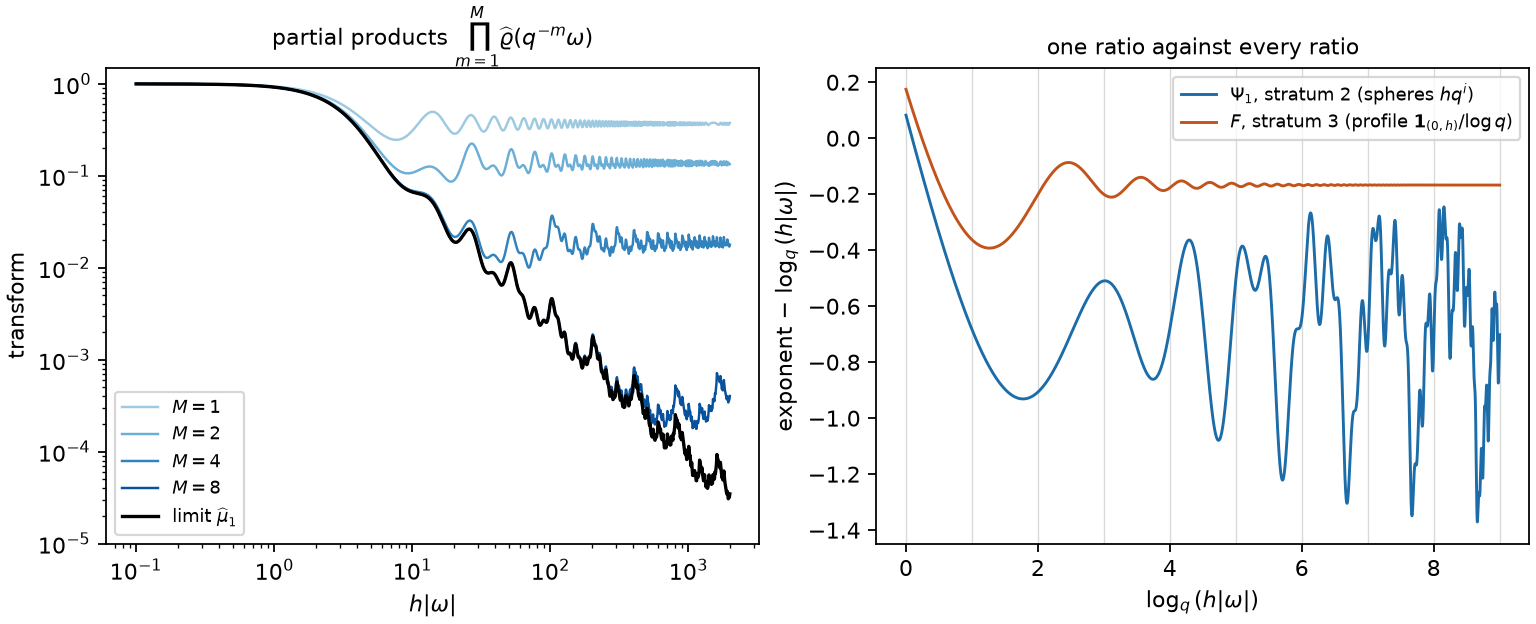
\includegraphics[width=\textwidth]{theory-strata.png}
\caption{The family of Proposition~\ref{prop:stratum-two-example} at $d = 2$, $q = 2$, $h = 1$,
with the weights $w_i = 1$ for $i < 0$ and $w_i = 0$ for $i \ge 0$ of the proof of
Theorem~\ref{thm:lattice-strata-strict}. Its ladder step $\varrho = \mu_{1,q}$ has the \Levy{}
measure $\sigma_h$, so $\widehat\varrho(\omega) = \exp\bigl(-(1 - J_0(h|\omega|))\bigr)$, where
$J_0 = \Omega_2$ is the Bessel function of order $0$. Left: the partial products of
Proposition~\ref{prop:ladder-knot-kernel}(1) for $M = 1, 2, 4, 8$, and their limit
$\widehat\mu_1$. At high frequency each factor tends to $e^{-1}$, so the $M$-th partial product
levels off near $e^{-M}$. Right, blue: $P(\omega) := \Psi_1(\omega) - \log_q(h|\omega|)$, with
$\Psi_1$ the exponent of the knot kernel. It satisfies $P(q\omega) - P(\omega) = -J_0(h|\omega|)$.
Since $|J_0(x)| \le Cx^{-1/2}$, these differences are summable along each ray $q^n\omega$, so $P$
converges to a function of period $1$ in $\log_q(h|\omega|)$. That this limit is not constant is
read from the plot. Orange: the same difference for the exponent $F(|\omega|)$ of the isotropic
origin datum $(0, (\log q)^{-1}\mathbf 1_{(0,h)})$, which spreads the same jumps evenly in $\log$
length. It lies in $\mathcal{A}_2$ (Theorem~\ref{thm:cited-A35}), and its difference tends to a
constant. The blue sum is cut at $m \le 89$. The orange integral is a trapezoid rule on
$4 \times 10^6$ steps of $[0, 1.001\,r_{\max}]$, with $r_{\max} = h q^9$ the largest frequency
plotted. The script \texttt{scripts/make\_figures\_theory.py} draws the figure.}
\label{fig:theory-strata}
\end{figure}

In clause (3), ``almost every $\omega$'' cannot be replaced by ``every $\omega \ne 0$'', as the next
example shows.

% shared with blueprint prop:ladder-not-every-frequency
\begin{proposition}[the partial products at one frequency]
\label{prop:ladder-not-every-frequency}

Let $d = 1$ and $q = 2$, and let $\varrho$ be the compound Poisson law on $\ZZ$ with the \Levy{}
measure $\nu_\varrho := \sum_{j \ge 1}j^{-2}\cdot\tfrac12(\delta_{2^j} + \delta_{-2^j})$, whose folded
\Levy{} measure is $\sum_{j \ge 1}j^{-2}\delta_{2^j}$. Then $\int\log_+|x|\,\nu_\varrho(dx) = \infty$,
and the partial products $\prod_{m=1}^M\widehat\varrho(2^{-m}\omega)$ have a positive limit at
$\omega = 2\pi$.
\end{proposition}

\begin{proof}
The measure $\nu_\varrho$ is symmetric with total mass $c := \sum_jj^{-2} < \infty$. Let
$\varrho := e^{-c}\sum_{n \ge 0}\nu_\varrho^{*n}/n!$, the law of $Y_1 + \dots + Y_N$ with $N$ Poisson
of mean $c$ and $Y_1, Y_2, \dots$ independent with law $\nu_\varrho/c$, independent of $N$. It is a
probability law with $\widehat\varrho = e^{-c}\exp\widehat{\nu_\varrho}$, and since $\nu_\varrho$ is
symmetric, $\widehat{\nu_\varrho}(\omega) = \int\cos\omega x\,\nu_\varrho(dx)$, so
$\widehat\varrho(\omega) = \exp\bigl(-\int(1 - \cos\omega x)\,\nu_\varrho(dx)\bigr)
= \exp\bigl(-\sum_jj^{-2}(1 - \cos(2^j\omega))\bigr)$. A law with this transform is $\varrho$, the
transform determining the law. It is carried by $\ZZ$: so is $\nu_\varrho$, and a convolution of two
measures carried by $\ZZ$ is carried by $\ZZ$, so every $\nu_\varrho^{*n}$ is. It is infinitely
divisible: for $n \ge 1$ the compound Poisson law of $\nu_\varrho/n$ has the transform
$\widehat\varrho^{1/n}$, so its $n$-th convolution power is $\varrho$. The moment fails:
$\int\log_+|x|\,\nu_\varrho(dx) = \sum_jj^{-2}\cdot j\log 2 = \infty$, the harmonic series diverging.
At $\omega = 2\pi$,
\[
  -\log\prod_{m=1}^M\widehat\varrho(2^{-m}\cdot2\pi) = \sum_{m=1}^M\sum_{j \ge 1}j^{-2}\bigl(1 - \cos(2\pi2^{j-m})\bigr).
\]
The terms with $m \le j$ vanish, since $2^{j-m}$ is an integer. Writing $i := m - j \ge 1$ for the
others, the double sum increases with $M$ to
\[
  \sum_{m \ge 1}\sum_{j \ge 1}j^{-2}\bigl(1 - \cos(2\pi2^{j-m})\bigr) = \Bigl(\sum_{j \ge 1}j^{-2}\Bigr)
  \sum_{i \ge 1}\bigl(1 - \cos(2\pi2^{-i})\bigr) < \infty,
\]
since $1 - \cos u \le u^2/2$ makes the last series at most $\sum_i2\pi^24^{-i}$. (The sums are of
nonnegative terms, so they may be taken over $m$ for each $j$ first.) So the partial products at
$2\pi$ decrease to the positive limit $\exp\bigl(-\sum_m\sum_jj^{-2}(1 - \cos(2\pi2^{j-m}))\bigr)$.

Every step is machine-checked, with no cited fact.
\end{proof}

In sum, the ladder fixes the knot kernels, and the families through one ladder differ only between
the knots. A symmetric infinitely divisible law other than a point mass is the step $\mu_{1,q}$ of a
symmetric $q$-covariant family in the canonical discrete gauge exactly when it has the logarithmic
moment (clauses (1) and (2)). This sorts the masks of grid pyramids. A symmetric infinitely
divisible mask $\varrho \ne \delta_0$ on a full-rank lattice with the moment is the step of a
pyramid strictly in stratum~2, and of no family in stratum~3 (clause (4)(a)). A finite mask other
than a point mass is the step of no family at all, as the next subsection shows.

\subsection{Steps of bounded support}
\label{sec:pyramid-bounded}

This last subsection returns to the classical pyramids. They smooth with a finite mask, applied
separably [\sscite{burt1983laplacian}, p.~533]. The mask is a five-tap mask of Burt's family or a
B-spline mask. The binomial $\tfrac1{16}[1,4,6,4,1]$ is in Burt's family
[\sscite{burt1981fast}, p.~24]. No such mask is a step of any family that is continuous in scale,
whatever its symmetry or covariance. The proposition joins two facts of probability theory: the
increments of an additive process in law are infinitely divisible [\sscite{sato1999levy},
Thm.~9.1, p.~47], and an infinitely divisible law other than a point mass has unbounded support
(Theorem~\ref{thm:cited-A46}).

% shared with blueprint prop:no-bounded-step
\begin{proposition}[no continuous family has a step of bounded support]
\label{prop:no-bounded-step}

Let $w$ be a probability measure on $\RR^d$ with bounded support, not a point mass. Then $w$ is not
infinitely divisible. So $w$ is no $\mu_{s,t}$ of any family of probability measures on $\RR^d$ with
(I1) and (I2), with no assumption of symmetry, rotation invariance, covariance or (ND).
\end{proposition}

\begin{proof}
By Theorem~\ref{thm:cited-A46}, an infinitely divisible law on $\RR^d$ that is not a point mass
has unbounded support. This is the first sentence. For the second, let $(\mu_{s,t})$ satisfy (I1)
and (I2). By Lemma~\ref{lem:steps-infinitely-divisible} every $\mu_{s,t}$ is infinitely
divisible. So $w$, which is not, is no $\mu_{s,t}$.

Every step is machine-checked, and the cited facts are \ledger{A46} and, through
Lemma~\ref{lem:steps-infinitely-divisible}, \ledger{A41}.
\end{proof}

This excludes the binomial mask, its tensor powers and the B-spline masks, on the continuum and on
any grid. The exclusion rests on continuity in scale. If only the levels are looked at, a finite
mask can behave like a step. A law $\mu$ is \emph{refinable} if it satisfies the \emph{knot
relation} $D_q\mu = \mu * w$ for some law $w$, the mask. Its dilate is then the law itself smoothed
by $w$, which is what a step does to a knot kernel. The word is that of subdivision, where a
function $\phi$ with $\phi(x) = \sum_k a_k\phi(2x - k)$ is called refinable
[\sscite{cavaretta1991stationary}, (1.7), pp.~4--5].
On the line the knot relation says that $X$ and $q^{-1}X + q^{-1}Y$ have one law, with $Y$ of law $w$
independent of $X$. By Vervaat's theorem on this equation a solution exists exactly when
$E\log_+|Y| < \infty$ [\sscite{vervaat1979stochastic}, Thm.~1.6(b), p.~757]. So a mask on the line
has a refinable law exactly when it has a logarithmic moment, whether or not it is infinitely
divisible.
Clause (2) of the next proposition shows that the binomial mask has a refinable law, the cubic
B-spline. The convergence belongs to subdivision theory. The scheme of a nonnegative mask converges
under the support condition of [\sscite{cavaretta1991stationary}, Thm.~3.3, p.~48], which the
B-spline masks meet, and the B-splines satisfy the refinement equation of their masks
[\sscite{cavaretta1991stationary}, p.~161]. Clause (2) proves the case at
hand by Vi\`ete's product and reads the limit as a refinable law, a solution of the knot relation
that is the knot kernel of no family. Clause (1) reads Burt's observation that the rescaled equivalent weights approach one
shape [\sscite{burt1981fast}, Obs.~1, p.~24]. The shape is approached and never reached, since no
equivalent weight is the $q$-dilate of the one before. That clause holds for every $q > 0$, though
a pyramid has $q > 1$.

% shared with blueprint prop:equivalent-weights
\begin{proposition}[equivalent weights and the knot relation]
\label{prop:equivalent-weights}

Let $w$ be a law on $\RR^d$, $q > 0$, and $W_n := w * D_qw * \dots * D_{q^{n-1}}w$ the equivalent
weight at level $n$, with $W_0 := \delta_0$.
\begin{enumerate}
\item If $w \ne \delta_0$, then $W_n \ne D_qW_{n-1}$ for every $n \ge 1$: no equivalent weight is the
$q$-dilate of the one before it, for any mask, symmetric or not, infinitely divisible or not.
\item A finite mask can satisfy the knot relation. For instance, let $q = 2$ and let $w$ be the
binomial mask on $h\ZZ$,
\[
  w = \tfrac1{16}\bigl(\delta_{-2h} + 4\delta_{-h} + 6\delta_0 + 4\delta_h + \delta_{2h}\bigr).
\]
The law $\mu_1$ with
$\widehat\mu_1(\omega) = \prod_{m \ge 1}\widehat w(2^{-m}\omega) = \bigl(\sin(h\omega/2)/(h\omega/2)\bigr)^4$,
the cubic B-spline, has $D_2\mu_1 = \mu_1 * w$, and its tensor powers do the same on $h\ZZ^d$.
\end{enumerate}
\end{proposition}

\begin{proof}
(1) Write $P(\omega) := \widehat W_{n-1}(q\omega) = \prod_{k=1}^{n-1}\widehat w(q^k\omega)$, the
transform of $D_qW_{n-1}$. Since $W_n = w * D_qW_{n-1}$, the equation $W_n = D_qW_{n-1}$ would give
$\widehat w\,P = P$, that is $(1 - \widehat w)P = 0$. The function $P$ is continuous with
$P(0) = 1$, so it has no zero on a ball $B_\eta$ about $0$, and $\widehat w = 1$ on $B_\eta$.

A probability measure $w$ with $\widehat w = 1$ on $B_\eta$ is $\delta_0$. Indeed, if
$\widehat w(\omega) = 1$, then $\int(1 - \cos\langle\omega, x\rangle)\,w(dx) = 0$, and the integrand
is nonnegative, so $\cos\langle\omega, x\rangle = 1$ for $w$-almost every $x$. Let $b_1, \dots, b_d$
be a basis and $c > 0$ with $c|b_j| < \eta$ for every $j$. Applying this at the countably many points
$c\,b_j/m$, $m \ge 1$, gives a $w$-null set off which $\cos(c\langle b_j, x\rangle/m) = 1$ for every
$j$ and every $m$. A real number $\theta$ with $\cos(\theta/m) = 1$ for every $m \ge 1$ is $0$,
since $|\theta/m| < 2\pi$ for $m$ large. So $\langle b_j, x\rangle = 0$ for every $j$, that is $x = 0$,
for $w$-almost every $x$, and $w = \delta_0$. This contradicts $w \ne \delta_0$. At $n = 1$ the
product $P$ is empty and equals $1$.

(2) The transform of the mask is
$\widehat w(\omega) = \tfrac1{16}(e^{-ih\omega/2} + e^{ih\omega/2})^4 = \cos^4(h\omega/2)$. Write
$\operatorname{sinc} x := \sin x/x$, with $\operatorname{sinc} 0 := 1$. Since
$\sin 2t = 2\sin t\cos t$, $\operatorname{sinc}(2t) = \operatorname{sinc}(t)\cos t$, and induction
on $M$ gives
\[
  \operatorname{sinc} x = \operatorname{sinc}(x2^{-M})\prod_{m=1}^{M}\cos(x2^{-m}) .
\]
As $\operatorname{sinc}$ is continuous with $\operatorname{sinc} 0 = 1$, the partial products tend
to $\operatorname{sinc} x$. At $x = h\omega/2$ this gives
$\prod_{m \ge 1}\widehat w(2^{-m}\omega) = (\sin(h\omega/2)/(h\omega/2))^4$. The uniform law on
$[-h/2, h/2]$ has the transform $\operatorname{sinc}(h\omega/2)$, so its fourfold convolution, the
cubic B-spline, has the transform of $\mu_1$. By the uniqueness of the transform it is the only
probability measure with that transform. Then
$\widehat\mu_1(2\omega) = \operatorname{sinc}(h\omega)^4
= \operatorname{sinc}(h\omega/2)^4\cos^4(h\omega/2) = \widehat\mu_1(\omega)\widehat w(\omega)$,
which is $D_2\mu_1 = \mu_1 * w$. For the tensor powers on $h\ZZ^d$ the transforms are products over
the coordinates, and $D_2$ acts on each factor.

Every step is machine-checked, with no cited fact.
\end{proof}

The cubic B-spline shows why Definition~\ref{def:self-decomposable} requires the residual to be
infinitely divisible. With any residual the class is wider. Maejima and Naito give it Lo\`eve's
name, $b$-decomposable, and note that its laws need not be infinitely divisible
[\sscite{maejima1998semi}, Rem.~3.1, pp.~19--20]. The B-spline is $b$-decomposable with $b = 2$. By
$D_2\mu_1 = \mu_1 * w$ it is the law of $\tfrac12X + Y$, with $X$ of that law and $Y$ of the law
$D_{1/2}w$, independent of $X$. Definition~\ref{def:self-decomposable} excludes it. The B-spline has bounded support and is
not a point mass, so it is not infinitely divisible (Proposition~\ref{prop:no-bounded-step}), while
a semi-selfdecomposable law is (Theorem~\ref{thm:cited-A43}). Section~\ref{sec:price-masks} reads
the same example on a grid, after Proposition~\ref{prop:exact-masks}.

